%% LyX 2.3.6.2 created this file.  For more info, see http://www.lyx.org/.
%% Do not edit unless you really know what you are doing.
\documentclass[english,dvipsnames,aspectratio=169,handout]{beamer}
\usepackage{mathptmx}
\usepackage{algorithm2e}
\usepackage{eulervm}
\usepackage[T1]{fontenc}
\usepackage[latin9]{inputenc}
\usepackage{babel}
\usepackage{amstext}
\usepackage{amssymb}
\usepackage{graphicx}
\usepackage{ifthen}
\usepackage{xcolor}
\usepackage{comment}
\usepackage{xspace}
\usepackage{tikz}
\usetikzlibrary{tikzmark}
\usetikzlibrary{calc}
\usepackage{pgfplots}
\usepackage{booktabs}
\usepackage{xpatch}
\usepackage{multirow}
\usepackage{colortbl}
\usepackage{pgfpages}
\usepackage{bbm}


\ifx\hypersetup\undefined
  \AtBeginDocument{%
    \hypersetup{unicode=true,pdfusetitle,
 bookmarks=true,bookmarksnumbered=false,bookmarksopen=false,
 breaklinks=false,pdfborder={0 0 0},pdfborderstyle={},backref=false,colorlinks=true,
 allcolors=NYUPurple,urlcolor=LightPurple}
  }
\else
  \hypersetup{unicode=true,pdfusetitle,
 bookmarks=true,bookmarksnumbered=false,bookmarksopen=false,
 breaklinks=false,pdfborder={0 0 0},pdfborderstyle={},backref=false,colorlinks=true,
 allcolors=NYUPurple,urlcolor=LightPurple}
\fi

\makeatletter


%%%%%%%%%%%%%%%%%%%%%%%%%%%%%% LyX specific LaTeX commands.
%% Because html converters don't know tabularnewline
\providecommand{\tabularnewline}{\\}

% %%%%%%%%%%%%%%%%%%%%%%%%%%%%%% Textclass specific LaTeX commands.
% % this default might be overridden by plain title style
% \newcommand\makebeamertitle{\frame{\maketitle}}%
% % (ERT) argument for the TOC
% \AtBeginDocument{%
%   \let\origtableofcontents=\tableofcontents
%   \def\tableofcontents{\@ifnextchar[{\origtableofcontents}{\gobbletableofcontents}}
%   \def\gobbletableofcontents#1{\origtableofcontents}
% }

%%%%%%%%%%%%%%%%%%%%%%%%%%%%%% User specified LaTeX commands.
\usetheme{CambridgeUS} 
\beamertemplatenavigationsymbolsempty


% Set Color ==============================
\definecolor{NYUPurple}{RGB}{87,6,140}
\definecolor{LightPurple}{RGB}{165,11,255}


\setbeamercolor{title}{fg=NYUPurple}
%\setbeamercolor{frametitle}{fg=NYUPurple}
\setbeamercolor{frametitle}{fg=NYUPurple}

\setbeamercolor{background canvas}{fg=NYUPurple, bg=white}
\setbeamercolor{background}{fg=black, bg=NYUPurple}

\setbeamercolor{palette primary}{fg=black, bg=gray!30!white}
\setbeamercolor{palette secondary}{fg=black, bg=gray!20!white}
\setbeamercolor{palette tertiary}{fg=gray!20!white, bg=NYUPurple}

\setbeamertemplate{headline}{}

\setbeamercolor{parttitle}{fg=NYUPurple}
\setbeamercolor{sectiontitle}{fg=NYUPurple}
\setbeamercolor{sectionname}{fg=NYUPurple}
\setbeamercolor{section page}{fg=NYUPurple}

% \AtBeginSection[]{
%   \begin{frame}
%     \frametitle{Table of Contents}
%     \tableofcontents[currentsection]
%   \end{frame}

%   % \begin{frame}
%   % \vfill
%   % \centering
%   % \begin{beamercolorbox}[sep=8pt,center,shadow=true,rounded=true]{title}
%   %   \usebeamerfont{title}\insertsectionhead\par%
%   % \end{beamercolorbox}
%   % \vfill
%   % \end{frame}
% }

\makeatother

\begin{document}
\global\long\def\reals{\mathbf{R}}%
 
\global\long\def\integers{\mathbf{Z}}%
 
\global\long\def\naturals{\mathbf{N}}%
 
\global\long\def\rationals{\mathbf{Q}}%
 
\global\long\def\ca{\mathcal{A}}%
 
\global\long\def\cb{\mathcal{B}}%
 
\global\long\def\cc{\mathcal{C}}%
 
\global\long\def\cd{\mathcal{D}}%
 
\global\long\def\ce{\mathcal{E}}%
 
\global\long\def\cf{\mathcal{F}}%
 
\global\long\def\cg{\mathcal{G}}%
 
\global\long\def\ch{\mathcal{H}}%
 
\global\long\def\ci{\mathcal{I}}%
 
\global\long\def\cj{\mathcal{J}}%
 
\global\long\def\ck{\mathcal{K}}%
 
\global\long\def\cl{\mathcal{L}}%
 
\global\long\def\cm{\mathcal{M}}%
 
\global\long\def\cn{\mathcal{N}}%
 
\global\long\def\co{\mathcal{O}}%
 
\global\long\def\cp{\mathcal{P}}%
 
\global\long\def\cq{\mathcal{Q}}%
 
\global\long\def\calr{\mathcal{R}}%
 
\global\long\def\cs{\mathcal{S}}%
 
\global\long\def\ct{\mathcal{T}}%
 
\global\long\def\cu{\mathcal{U}}%
 
\global\long\def\cv{\mathcal{V}}%
 
\global\long\def\cw{\mathcal{W}}%
 
\global\long\def\cx{\mathcal{X}}%
 
\global\long\def\cy{\mathcal{Y}}%
 
\global\long\def\cz{\mathcal{Z}}%
 
\global\long\def\ind#1{\mathbbm{1}[#1]}%
 %\newcommand{\pr}{P}
\global\long\def\pr{\mathbb{P}}%
 
\global\long\def\predsp{\cy}%
 %{\hat{\cy}}
\global\long\def\outsp{\cy}%

\global\long\def\prxy{P_{\cx\times\cy}}%
 
\global\long\def\prx{P_{\cx}}%
 
\global\long\def\prygivenx{P_{\cy\mid\cx}}%
 %\newcommand{\ex}{E}
\global\long\def\ex{\mathbb{E}}%
 
\global\long\def\var{\textrm{Var}}%
 
\global\long\def\cov{\textrm{Cov}}%
 
\global\long\def\sgn{\textrm{sgn}}%
 
\global\long\def\sign{\textrm{sign}}%
 
\global\long\def\kl{\textrm{KL}}%
 
\global\long\def\law{\mathcal{L}}%
 
\global\long\def\eps{\varepsilon}%
 
\global\long\def\as{\textrm{ a.s.}}%
 
\global\long\def\io{\textrm{ i.o.}}%
 
\global\long\def\ev{\textrm{ ev.}}%
 
\global\long\def\convd{\stackrel{d}{\to}}%
 
\global\long\def\eqd{\stackrel{d}{=}}%
 
\global\long\def\del{\nabla}%
 
\global\long\def\loss{\ell}%
 
\global\long\def\risk{R}%
 
\global\long\def\emprisk{\hat{R}}%
 
\global\long\def\lossfnl{L}%
 
\global\long\def\emplossfnl{\hat{L}}%
 
\global\long\def\empminimizer#1{\hat{#1}^{*}}%
 
\global\long\def\minimizer#1{#1^{*}}%
\global\long\def\optimizer#1{#1^{*}}%
 
\global\long\def\etal{\textrm{et. al.}}%
 
\global\long\def\tr{\operatorname{tr}}%

\global\long\def\trace{\operatorname{trace}}%
 
\global\long\def\diag{\text{diag}}%
 
\global\long\def\rank{\text{rank}}%
 
\global\long\def\linspan{\text{span}}%
 
\global\long\def\spn{\text{span}}%
 
\global\long\def\proj{\text{Proj}}%
 
\global\long\def\argmax{\operatornamewithlimits{arg\, max}}%
 
\global\long\def\argmin{\operatornamewithlimits{arg\, min}}%

\global\long\def\bfx{\mathbf{x}}%
 
\global\long\def\bfy{\mathbf{y}}%
 
\global\long\def\bfl{\mathbf{\lambda}}%
 
\global\long\def\bfm{\mathbf{\mu}}%
 
\global\long\def\calL{\mathcal{L}}%

\global\long\def\vw{\boldsymbol{w}}%
 
\global\long\def\vx{\boldsymbol{x}}%
 
\global\long\def\vxi{\boldsymbol{\xi}}%
 
\global\long\def\valpha{\boldsymbol{\alpha}}%
 
\global\long\def\vbeta{\boldsymbol{\beta}}%
 
\global\long\def\vsigma{\boldsymbol{\sigma}}%
\global\long\def\vtheta{\boldsymbol{\theta}}%
 
\global\long\def\vd{\boldsymbol{d}}%
 
\global\long\def\vs{\boldsymbol{s}}%
 
\global\long\def\vt{\boldsymbol{t}}%
 
\global\long\def\vh{\boldsymbol{h}}%
 
\global\long\def\ve{\boldsymbol{e}}%
 
\global\long\def\vf{\boldsymbol{f}}%
 
\global\long\def\vg{\boldsymbol{g}}%
 
\global\long\def\vz{\boldsymbol{z}}%
 
\global\long\def\vk{\boldsymbol{k}}%
 
\global\long\def\va{\boldsymbol{a}}%
 
\global\long\def\vb{\boldsymbol{b}}%
 
\global\long\def\vv{\boldsymbol{v}}%
 
\global\long\def\vy{\boldsymbol{y}}%

\global\long\def\dom{\textrm{\textbf{dom} }}%
\global\long\def\rank{\text{\textbf{rank }}}%
\global\long\def\conv{\textrm{\textbf{conv} }}%
\global\long\def\relint{\text{\textbf{relint }}}%
\global\long\def\aff{\text{\textbf{aff }}}%

\global\long\def\hil{\ch}%
 
\global\long\def\rkhs{\hil}%
 
\global\long\def\ber{\text{Ber}}%

\global\long\def\softmax{\text{Softmax}}%

\title[DS-GA 1003 ]{Probabilistic models - Bayesian Methods}
\author{Mengye Ren}
% \author{Tal Linzen \\
% Slides based on Lecture
% \href{https://github.com/davidrosenberg/mlcourse/blob/gh-pages/Lectures/08a.bayesian-methods.pdf}{08a} from David Rosenberg's course materials (\url{https://github.com/davidrosenberg/mlcourse}) and Marylou Gabri\'e's materials
% }
\date{Oct 31, 2023}
\institute{NYU}

% \title[DS-GA 1003]{Bayesian Methods}
% \author{Julia Kempe \& David S. Rosenberg }
% \date{March 26, 2019}
% \institute{CDS, NYU}

% \makebeamertitle
\maketitle
\mode<article>{Just in article version}


\section{Bayesian ML: Classical Statistics}
\begin{frame}{Parametric Family of Densities}
\begin{itemize}
\item A \textbf{parametric family of densities }is a set 
\[
\left\{ p(y\mid\theta):\theta\in\Theta\right\} ,
\]


\begin{itemize}
\item where $p(y\mid\theta)$ is a density on a \textbf{sample space }$\cy$,
and
\item $\theta$ is a \textbf{parameter} in a {[}finite dimensional{]} \textbf{parameter
space $\Theta$.}
\end{itemize}
\end{itemize}

\pause{}
\begin{itemize}
\item This is the common starting point for a treatment of classical or
Bayesian statistics.
\item In this lecture, whenever we say ``density'', we could replace it
    with ``mass function.'' (and replace integrals with sums).{\scriptsize{} }{\scriptsize\par}
\end{itemize}
\end{frame}

\begin{frame}{Frequentist or ``Classical'' Statistics}
\begin{itemize}
\item We're still working with a parametric family of densities:
\[
\left\{ p(y\mid\theta)\mid\theta\in\Theta\right\} .
\]
\end{itemize}

\pause{}
\begin{itemize}
\item Assume that $p(y\mid\theta)$ governs the world we are observing,
for some $\theta\in\Theta$.
\end{itemize}

\pause{}
\begin{itemize}
\item If we knew the right $\theta\in\Theta$, there would be no need for
statistics.
\end{itemize}

\pause{}
\begin{itemize}
\item But instead of $\theta$, we have data $\cd$: $y_{1},\ldots,y_{n}$ sampled
i.i.d. from $p(y\mid\theta)$.
\end{itemize}

\pause{}
\begin{itemize}
\item Statistics is about how to get by with $\cd$ in place of $\theta$.
\end{itemize}
\end{frame}
%

\begin{frame}{Point Estimation}

\begin{itemize}
\item One type of statistical problem is\textbf{ point estimation}.
\end{itemize}

\pause{}
\begin{itemize}
\item A \textbf{statistic} $s=s(\cd)$ is any function of the data.
\end{itemize}

\pause{}
\begin{itemize}
\item A statistic $\hat{\theta}=\hat{\theta}(\cd)$ taking values in $\Theta$
is a\textbf{ point estimator of} $\theta$.
\end{itemize}

\pause{}
\begin{itemize}
\item A good point estimator will have $\hat{\theta}\approx\theta$.
% \end{itemize}
% \end{frame}
% %
% \begin{frame}{Desirable Properties of Point Estimators}
% \begin{itemize}
\item \textbf{Desirable statistical properties of point estimators}:

\pause{}
\begin{itemize}
\item \textbf{Consistency: }As data size $n\to\infty$, we get $\hat{\theta}_{n}\to\theta$.
\end{itemize}

\pause{}
\begin{itemize}
\item \textbf{Efficiency:} (Roughly speaking) $\hat{\theta}_{n}$ is as
accurate as we can get from a sample of size $n$.
\end{itemize}
\end{itemize}


\pause{}
\begin{itemize}
\item \textbf{Maximum likelihood estimators }are consistent and efficient
under reasonable conditions.
\end{itemize}
\end{frame}
%
% \begin{frame}{The Likelihood Function}
% \begin{itemize}
% \item Consider parametric family $\left\{ p(y\mid\theta):\theta\in\Theta\right\} $
% and i.i.d. sample $\cd=\left(y_{1},\ldots,y_{n}\right)$.

% \pause{}
% \item The density for sample $\cd$ for $\theta\in\Theta$ is
% \[
% p(\cd\mid\theta)\pause=\prod_{i=1}^{n}p(y_{i}\mid\theta).
% \]


% \pause{}
% \item $p(\cd\mid\theta)$ is a function of $\cd$ and $\theta$. 

% \pause{}
% \item For fixed $\theta$, $p(\cd\mid\theta$) is a density function on
% $\cy^{n}$.

% \pause{}
% \item For fixed $\cd$, the function $\theta\mapsto p(\cd\mid\theta)$ is
% called the \textbf{likelihood function:
% \[
% L_{\cd}(\theta):=p(\cd\mid\theta).
% \]
% }
% \end{itemize}
% \end{frame}
% %
% \begin{frame}{Maximum Likelihood Estimation}
% \begin{definition}
% The \textbf{maximum likelihood estimator (MLE)} for $\theta$ in the
% model $\left\{ p(y\mid\theta):\theta\in\Theta\right\} $ is
% \begin{eqnarray*}
% \hat{\theta}_{\text{MLE}} & = & \argmax_{\theta\in\Theta}L_{\cd}(\theta).
% \end{eqnarray*}

% \pause{}
% \end{definition}

% \begin{itemize}
% \item Maximum likelihood is just one approach to getting a point estimator
% for $\theta$.

% \pause{}
% \item \textbf{Method of moments} is another general approach one learns
% about in statistics.

% \pause{}
% \item Later we'll talk about \textbf{MAP }and \textbf{posterior mean }as
% approaches to point estimation.
% \begin{itemize}
% \item These arise naturally in Bayesian settings.
% \end{itemize}
% \end{itemize}
% \end{frame}
%
\begin{frame}{Example of Point Estimation: Coin Flipping}
\begin{itemize}
\item Parametric family of mass functions:
\[
p(\text{Heads}\mid\theta)=\theta,
\]
for $\theta\in\Theta=\left(0,1\right)$.
\end{itemize}
\end{frame}
%
\begin{frame}{Coin Flipping: MLE}
\begin{itemize}
\item Data $\cd=\left(H,H,T,T,T,T,T,H,\ldots,T\right)$, assumed i.i.d. flips.
\begin{itemize}
\item $n_{h}$: number of heads
\item $n_{t}$: number of tails\textbf{ }
\end{itemize}
% \item 

\pause{}
\item \textbf{Likelihood function }for data $\cd$:

\[
L_{\cd}(\theta)=\pause p(\cd\mid\theta)=\theta^{n_{h}}\left(1-\theta\right)^{n_{t}}
\]

% \pause{}
% \item (This is the probability of getting the flips in the order they were
% received)
% \end{itemize}
% \end{frame}
%
% \begin{frame}{Coin Flipping: MLE}
 
% \begin{itemize}
\item As usual, it is easier to maximize the log-likelihood function:
\begin{eqnarray*}
\hat{\theta}_{\text{MLE}} & = & \argmax_{\theta\in\Theta}\log L_{\cd}(\theta)\\
 & = & \argmax_{\theta\in\Theta}\left[n_{h}\log\theta+n_{t}\log(1-\theta)\right]
\end{eqnarray*}
\end{itemize}

\pause{}
\begin{itemize}
    \item First order condition (equating the derivative to zero):
\[
\frac{n_{h}}{\theta}-\frac{n_{t}}{1-\theta} = 0 \iff\theta  =  \frac{n_{h}}{n_{h}+n_{t}} \pause \quad \quad  \hat{\theta}_{\text{MLE}} \text{ is the empirical fraction of heads.}
\]
% \item So $\hat{\theta}_{\text{MLE}}$ 
\end{itemize}
\end{frame}

\section{Bayesian Statistics: Introduction}
\begin{frame}{Bayesian Statistics}
 

\begin{itemize}
\item Baysian statistics introduces a crucial new ingredient: the \textbf{prior distribution.}
\end{itemize}

\pause{}
\begin{itemize}
\item A \textbf{prior distribution} $p(\theta)$ is a distribution on the parameter
space $\Theta$.
\end{itemize}

\pause{}
\begin{itemize}
\item The prior reflects our belief about $\theta$, \textbf{before seeing
any data}.
\end{itemize}
\end{frame}
%
\begin{frame}{A Bayesian Model }
\begin{itemize}
\item A {[}parametric{]} Bayesian model consists of two pieces:
\begin{enumerate}
\item A parametric family of densities 
\[
\left\{ p(\cd\mid\theta)\mid\theta\in\Theta\right\} .
\]


\pause{}
\item A \textbf{prior distribution} $p(\theta)$ on parameter space $\Theta$.

\pause{}
\end{enumerate}
\item Putting the pieces together, we get a joint density on $\theta$ and $\cd$:
\[
p(\cd,\theta)=p(\cd\mid\theta)p(\theta).
\]
\end{itemize}
\end{frame}
%
\begin{frame}{The Posterior Distribution}
\begin{itemize}
\item The \textbf{posterior distribution }for $\theta$ is $p(\theta\mid\cd)$.
\end{itemize}

\pause{}
\begin{itemize}
\item Whereas the prior represents belief about $\theta$ before observing data $\cd$,
\end{itemize}

\pause{}
\begin{itemize}
\item The posterior represents the\textbf{ rationally updated belief}
about $\theta$, after seeing $\cd$.
\end{itemize}
\end{frame}
%
\begin{frame}{Expressing the Posterior Distribution}
\begin{itemize}
\item By Bayes rule, can write the posterior distribution as
\[
p(\theta\mid\cd)\pause=\frac{p(\cd\mid\theta)p(\theta)}{p(\cd)}.
\]


\pause{}
\item Let's consider both sides as functions of $\theta$, for fixed $\cd$.

\pause{}
\item Then both sides are densities on $\Theta$ and we can write
\[
\underbrace{p(\theta\mid\cd)}_{\text{posterior}}\propto\underbrace{p(\cd\mid\theta)}_{\text{likelihood}}\underbrace{p(\theta)}_{\text{prior}}.
\]


\pause{}
\item Where $\propto$ means we've dropped factors that are independent of $\theta$. 
\end{itemize}
\end{frame}
%
\begin{frame}{Coin Flipping: Bayesian Model}
\begin{itemize}
\item Recall that we have a parametric family of mass functions:
\[
p(\text{Heads}\mid\theta)=\theta,
\]
for $\theta\in\Theta=\left(0,1\right)$.
\end{itemize}

\pause{}
\begin{itemize}
\item We need a prior distribution $p(\theta)$ on $\Theta=(0,1)$.
\end{itemize}

\pause{}
\begin{itemize}
\item One convenient choice would be a distribution from the Beta family
\end{itemize}
\end{frame}
%
\begin{frame}{Coin Flipping: Beta Prior}
\begin{itemize}
\item \textbf{Prior:}
\begin{eqnarray*}
\theta & \sim & \text{Beta}(\alpha,\beta)\\
p(\theta) & \propto & \theta^{\alpha-1}\left(1-\theta\right)^{\beta-1}
\end{eqnarray*}


\pause{}
\end{itemize}
\begin{center}
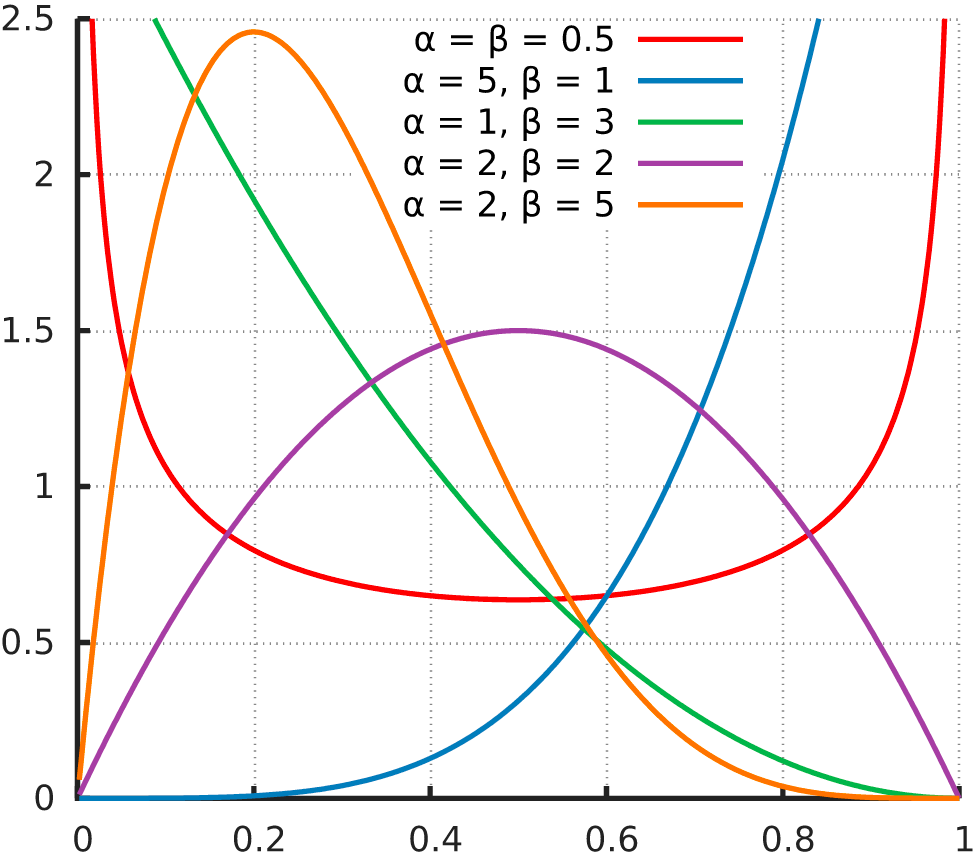
\includegraphics[height=0.55\textheight]{figures/betaFamily}
\par\end{center}


\let\thefootnote\relax\footnotetext{\tiny{Figure by Horas based on the work of Krishnavedala (Own work) [Public domain], via Wikimedia Commons \url{http://commons.wikimedia.org/wiki/File:Beta_distribution_pdf.svg}.}}
\end{frame}

%
\begin{frame}{Coin Flipping: Beta Prior}
\begin{itemize}
\item \textbf{Prior:}
\begin{eqnarray*}
\theta & \sim & \text{Beta}(h,t)\\
p(\theta) & \propto & \theta^{h-1}\left(1-\theta\right)^{t-1}
\end{eqnarray*}


\pause{}
\item \textbf{Mean of Beta distribution:} 
\[
\ex\theta=\frac{h}{h+t}
\]


\pause{}
\item \textbf{Mode of Beta distribution:} 
\[
\argmax_{\theta}p(\theta)=\frac{h-1}{h+t-2}
\]
for $h,t>1$.
\end{itemize}
\end{frame}
%
\begin{frame}{Coin Flipping: Posterior}
\begin{itemize}
\item \textbf{Prior:}
\begin{eqnarray*}
\theta & \sim & \text{Beta}(h,t)\\
p(\theta) & \propto & \theta^{h-1}\left(1-\theta\right)^{t-1}
\end{eqnarray*}
\end{itemize}

\pause{}
\begin{itemize}
\item \textbf{Likelihood function}
\[
L(\theta)=p(\cd\mid\theta)=\theta^{n_{h}}\left(1-\theta\right)^{n_{t}}
\]
\end{itemize}

\pause{}
\begin{itemize}
\item \textbf{Posterior density:}
\begin{eqnarray*}
p(\theta\mid\cd) & \propto & p(\theta)p(\cd\mid\theta)\\
\pause & \propto & \theta^{h-1}\left(1-\theta\right)^{t-1}\times\theta^{n_{h}}\left(1-\theta\right)^{n_{t}}\\
\pause & = & \theta^{h-1+n_{h}}\left(1-\theta\right)^{t-1+n_{t}}
\end{eqnarray*}
 
\end{itemize}
\end{frame}
%
\begin{frame}{The Posterior is in the Beta Family!}
\begin{itemize}
\item \textbf{Prior:}
\begin{eqnarray*}
\theta & \sim & \text{Beta}(h,t)\\
p(\theta) & \propto & \theta^{h-1}\left(1-\theta\right)^{t-1}
\end{eqnarray*}
 
\item \textbf{Posterior density:}
\begin{eqnarray*}
p(\theta\mid\cd) & \propto & \theta^{h-1+n_{h}}\left(1-\theta\right)^{t-1+n_{t}}
\end{eqnarray*}
\end{itemize}

\pause{}
\begin{itemize}
\item \textbf{Posterior is in the beta family}:
\begin{eqnarray*}
\theta\mid\cd & \sim & \text{Beta}(h+n_{h},t+n_{t})
\end{eqnarray*}
\end{itemize}

\pause{}
\begin{itemize}
\item \textbf{Interpretation}:
\begin{itemize}
\item Prior initializes our counts with $h$ heads and $t$ tails.
\item Posterior increments counts by observed $n_{h}$ and $n_{t}$. 
\end{itemize}
\end{itemize}
\end{frame}
%
\begin{frame}{Sidebar: Conjugate Priors}
\begin{itemize}
\item In this case, the posterior is in the same distribution family as the prior.
\item Let $\pi$ be a family of prior distributions on $\Theta$.

\pause{}
\item Let $P$ parametric family of distributions with parameter space $\Theta$.

\pause{}

\end{itemize}
\begin{definition}
A family of distributions \textbf{$\pi$ is conjugate to }parametric
model \textbf{$P$} if for any prior in $\pi$, the posterior is always
in $\pi$.

\pause{}
\end{definition}

\begin{itemize}
\item The beta family is conjugate to the coin-flipping (i.e. Bernoulli)
model.

%\pause{}
%\item The family of all probability distributions is conjugate to any parametric
%model. {[}Trvially{]}
\end{itemize}

\end{frame}
%
\begin{frame}{Coin Flipping: Concrete Example}
\begin{itemize}
\item Suppose we have a coin, possibly biased (\textbf{parametric probability
model}):
\[
p(\mbox{Heads}\mid\theta)=\theta.
\]


\pause{}
\item \textbf{Parameter space }$\theta\in\Theta=[0,1]$. 
\item \textbf{Prior distribution: }$\theta\sim\mbox{Beta}(2,2)$.

\pause{}
\end{itemize}
\begin{center}
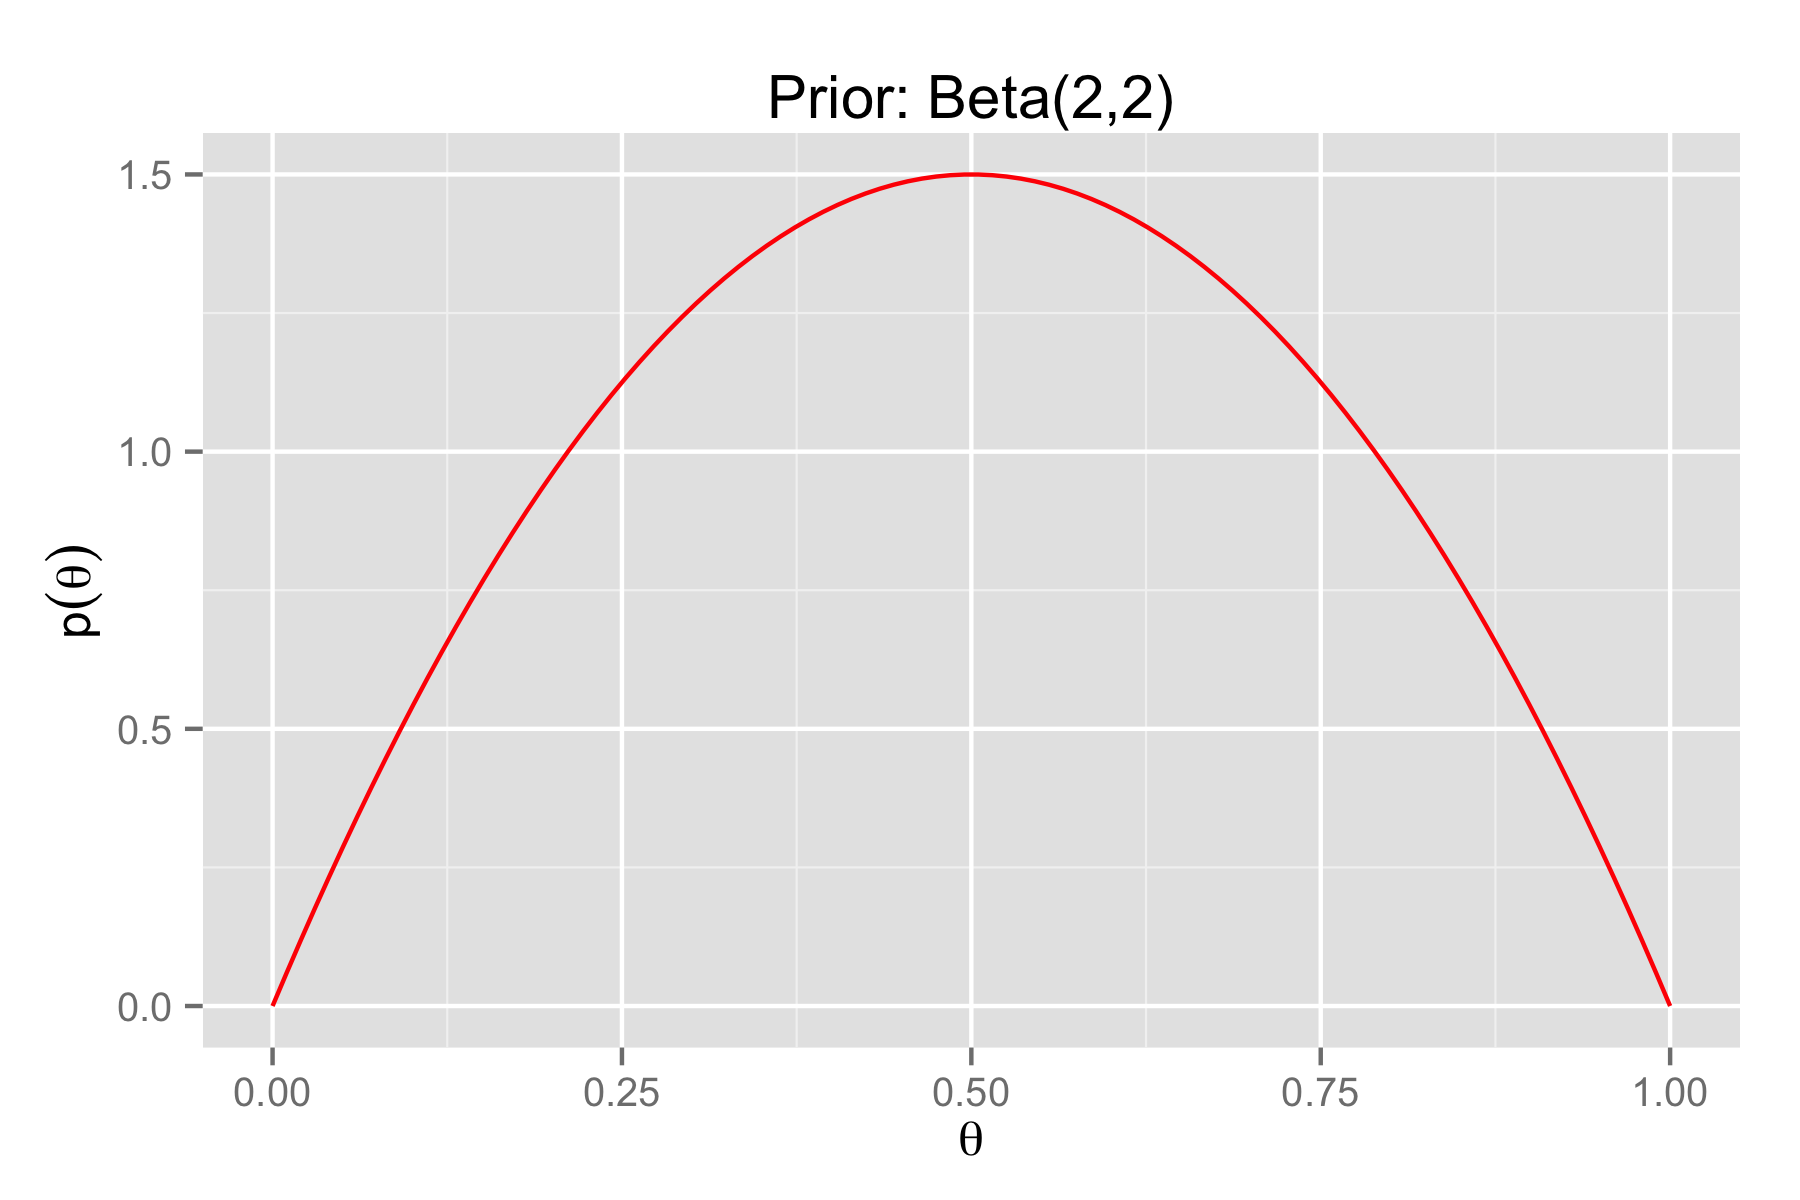
\includegraphics[height=0.5\textheight]{figures/beta2-2}
\par\end{center}

\end{frame}
%
\begin{frame}{Example: Coin Flipping}
\begin{itemize}
\item Next, we gather some data $\cd=\left\{ H,H,T,T,T,T,T,H,\ldots,T\right\} $:
\end{itemize}

\pause{}
\begin{itemize}
\item Heads: 75\qquad{}Tails: 60 

\pause{}
\begin{itemize}
\item $\hat{\theta}_{\text{MLE}}=\frac{75}{75+60}\approx0.556$

\pause{}
\end{itemize}
\item \textbf{Posterior distribution: $\theta\mid\cd\sim\mbox{Beta}(77,62)$:}
\end{itemize}
\begin{center}
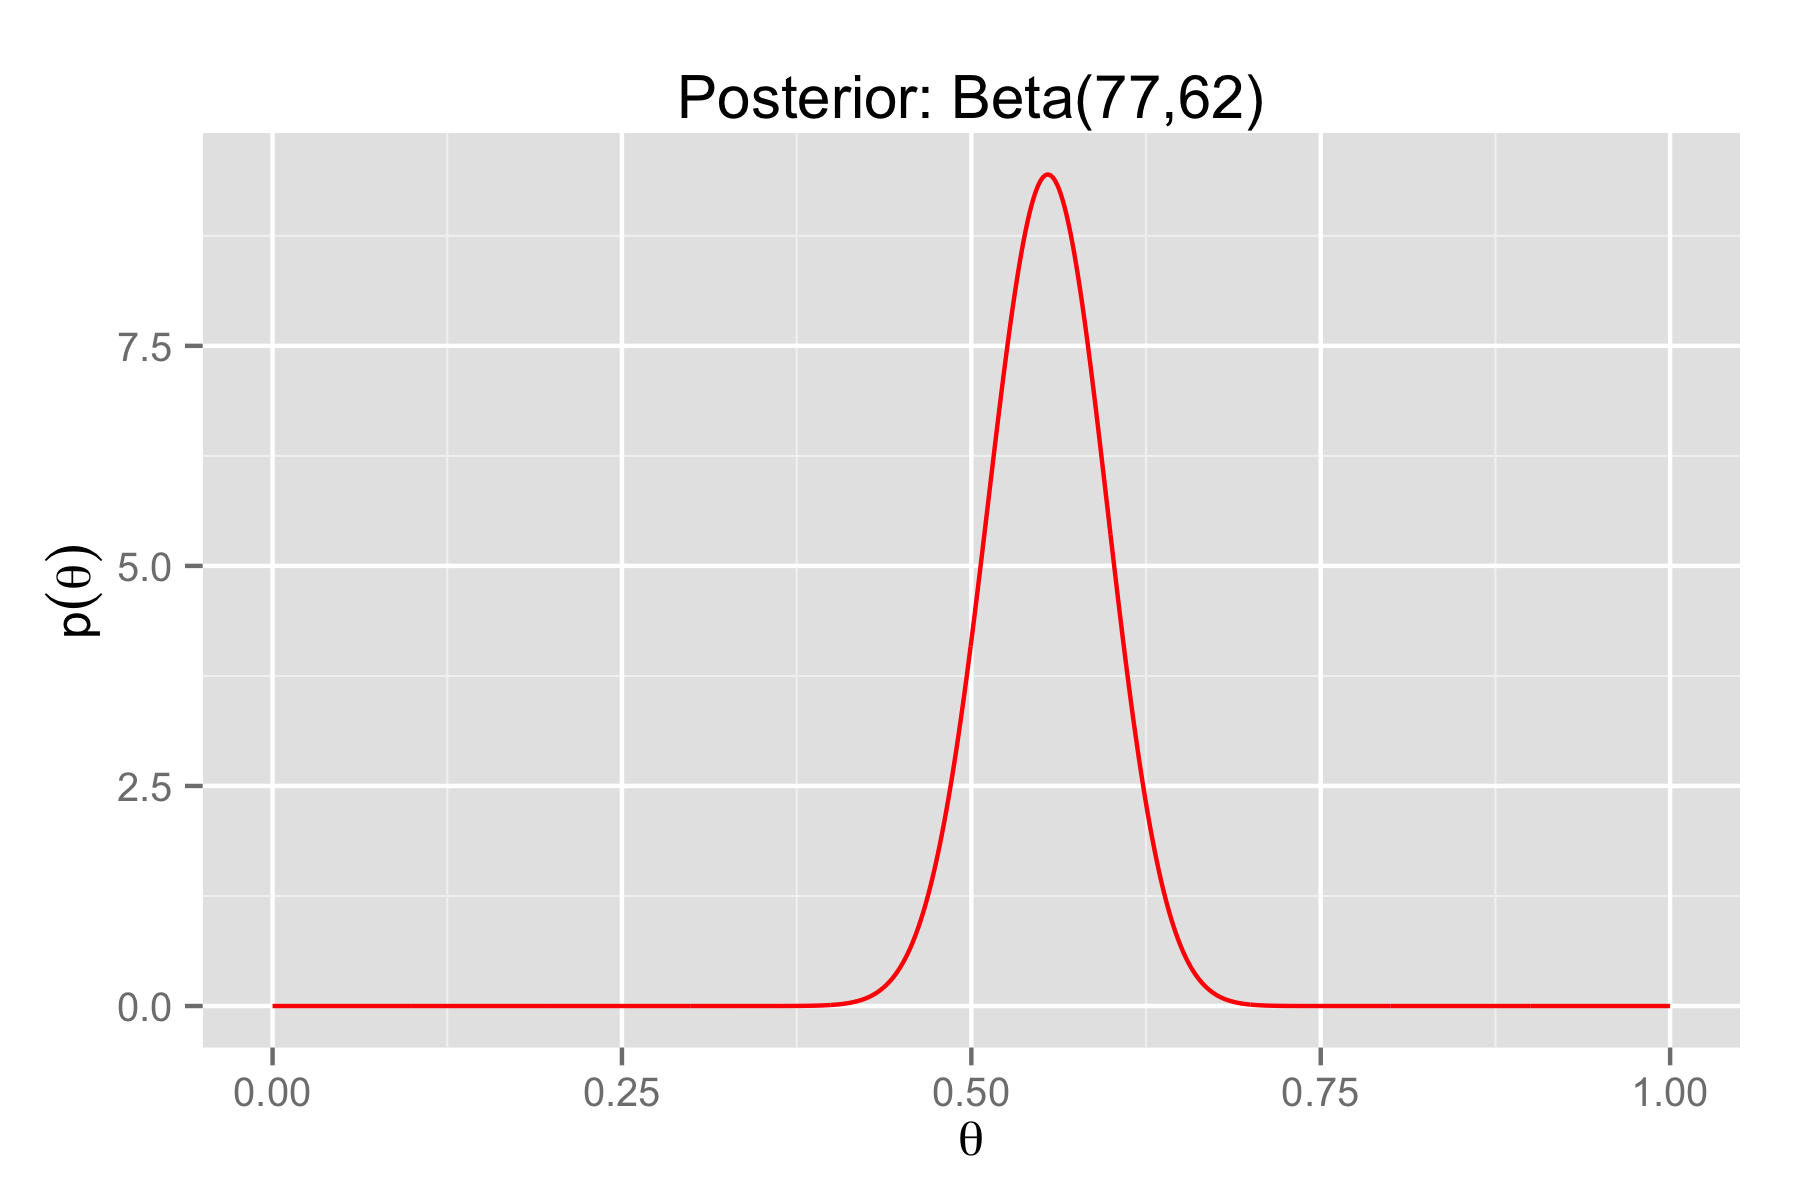
\includegraphics[height=0.6\textheight]{figures/beta77-62}
\par\end{center}

\end{frame}

\begin{frame}{Bayesian Point Estimates}
\begin{itemize}
\item We have the posterior distribution $\theta\mid\cd$.
\item What if someone asks us for a point estimate $\hat{\theta}$ for $\theta$?

\pause{}
\item Common options:

\pause{}
\begin{itemize}
\item \textbf{posterior mean} $\hat{\theta}=\ex\left[\theta\mid\cd\right]$

\pause{}
\item \textbf{maximum a posteriori (MAP) estimate} $\hat{\theta}=\argmax_{\theta}p(\theta\mid\cd)$ 
\begin{itemize}
\item Note: this is the \textbf{mode} of the posterior distribution
\end{itemize}
\end{itemize}
\end{itemize}
\end{frame}
%
\begin{frame}{What else can we do with a posterior?}
\begin{itemize}
\item Look at it: display uncertainty estimates to our client

\pause{}
\item Extract a \textbf{credible set} for $\theta$ (a Bayesian confidence
interval).
\begin{itemize}
\item e.g. Interval $[a,b]$ is a $95\%$\textbf{ credible set} if\textbf{
\[
\pr\left(\theta\in[a,b]\mid\cd\right)\ge0.95
\]
 }
\end{itemize}

\pause{}
\item Select a point estimate using \textbf{Bayesian decision theory}:
\begin{itemize}
\item Choose a loss function.
\item Find action \textbf{minimizing expected risk w.r.t. posterior}
\end{itemize}
\end{itemize}

\end{frame}

\section{Bayesian Decision Theory}
\begin{frame}{Bayesian Decision Theory}
\begin{itemize}
\item Ingredients: 
\begin{itemize}
\item \textbf{Parameter space} $\Theta$.
\item \textbf{Prior}: Distribution $p(\theta)$ on $\Theta$.
\item \textbf{Action space} $\ca$.
\item \textbf{Loss function}: $\ell:\ca\times\Theta\to\reals$.

\pause{}
\end{itemize}
\item The \textbf{posterior risk} of an action $a\in\ca$ is 
\begin{eqnarray*}
r(a) & := & \ex\left[\ell(\theta,a)\mid\cd\right]\\
\pause & = & \int\ell(\theta,a)p(\theta\mid\cd)\,d\theta.
\end{eqnarray*}


\pause{}
\begin{itemize}
\item It's the \textbf{expected loss under the posterior.}

\pause{}
\end{itemize}
\item A \textbf{Bayes action} $a^{*}$ is an action that minimizes posterior
risk:
\[
r(a^{*})=\min_{a\in\ca}r(a)
\]
\end{itemize}
\end{frame}
%
\begin{frame}{Bayesian Point Estimation}
\begin{itemize}
\item General Setup:
\begin{itemize}
\item Data $\cd$ generated by $p(y\mid\theta)$, for unknown $\theta\in\Theta$.

\pause{}
\item We want to produce a \textbf{point estimate} for $\theta$.

\pause{}
\end{itemize}
\item Choose:

\pause{}
\begin{itemize}
\item \textbf{Prior} $p(\theta)$ on $\Theta=\reals$.

\pause{}
\item \textbf{Loss} $\ell(\hat{\theta},\theta)$ %=\left(\theta-\hat{\theta}\right)^{2}$ 

\pause{}
\end{itemize}
\item Find \textbf{action} $\hat{\theta}\in\Theta$ that minimizes the \textbf{
posterior risk:}
\begin{eqnarray*}
r(\hat{\theta}) & = & \ex\left[\ell(\hat{\theta},\theta)\mid\cd\right]\\
\pause & = & \int\ell(\hat{\theta},\theta)p(\theta\mid\cd)\,d\theta
\end{eqnarray*}
\end{itemize}
\end{frame}
%
\begin{frame}{Important Cases}
\begin{itemize}
  \item Squared Loss :  $\ell(\hat{\theta},\theta)=\left(\theta-\hat{\theta}\right)^{2} \quad \Rightarrow$ posterior mean
  \item Zero-one Loss:  $\ell(\theta,\hat{\theta})=\ind{\theta\neq\hat{\theta}}\quad \Rightarrow $ posterior mode
  \item Absolute Loss :  $\ell(\hat{\theta},\theta)=\left|\theta-\hat{\theta}\right| \quad \Rightarrow$ posterior median
\end{itemize}

\pause
\begin{itemize}
    \item Optimal decision depends on the loss function and the posterior distribution.
    \item We will derive the square loss case next.
\end{itemize}
\end{frame}
%
\begin{frame}{Bayesian Point Estimation: Square Loss}
\begin{itemize}
\item Find \textbf{action} $\hat{\theta}\in\Theta$ that minimizes\textbf{
posterior risk} 
\begin{eqnarray*}
r(\hat{\theta}) & = & \int\left(\theta-\hat{\theta}\right)^{2}p(\theta\mid\cd)\,d\theta.
\end{eqnarray*}


\pause{}
\item Differentiate:
\end{itemize}
\begin{eqnarray*}
\frac{dr(\hat{\theta})}{d\hat{\theta}} & = & -\int2\left(\theta-\hat{\theta}\right)p(\theta\mid\cd)\,d\theta\\
\pause & = & -2\int\theta p(\theta\mid\cd)\,d\theta+2\hat{\theta}\underbrace{\int p(\theta\mid\cd)\,d\theta}_{=1}\\
\pause & = & -2\int\theta p(\theta\mid\cd)\,d\theta+2\hat{\theta}
\end{eqnarray*}

\end{frame}
%
\begin{frame}{Bayesian Point Estimation: Square Loss}
\begin{itemize}
\item Derivative of posterior risk is
\[
\frac{dr(\hat{\theta})}{d\hat{\theta}}=-2\int\theta p(\theta\mid\cd)\,d\theta+2\hat{\theta}.
\]


\pause{}
\item First order condition $\frac{dr(\hat{\theta})}{d\hat{\theta}}=0$
gives
\begin{eqnarray*}
\hat{\theta} & = & \int\theta p(\theta\mid\cd)\,d\theta\\
\pause & = & \ex\left[\theta\mid\cd\right]
\end{eqnarray*}
\end{itemize}

\pause{}
\begin{itemize}
\item The \textbf{Bayes action }for \textbf{square loss} is the posterior mean.
\end{itemize}
\end{frame}
%
% \begin{frame}{Bayesian Point Estimation: Absolute Loss}
% \begin{itemize}
% \item \textbf{Loss:}\emph{ $\ell(\theta,\hat{\theta})=\left|\theta-\hat{\theta}\right|$}

% \pause{}
% \item \textbf{Bayes action} for \textbf{absolute loss} is the \textbf{posterior
% median.}
% \begin{itemize}
% \item That is, the median of the distribution $p(\theta\mid\cd)$.

% \pause{}
% \item Show with approach similar to what was used in Homework \#1.
% \end{itemize}
% \end{itemize}
% \end{frame}
%
%\begin{frame}{Bayesian Point Estimation: Zero-One Loss}
%\begin{itemize}
%\item Suppose $\Theta$ is discrete (e.g. $\Theta=\left\{ \mbox{english},\mbox{french}\right\} $)
%\item \textbf{Zero-one loss:}\emph{ $\ell(\theta,\hat{\theta})=\ind{\theta\neq\hat{\theta}}$}

%\pause{}
%\item \textbf{Posterior risk}:
%\begin{eqnarray*}
%r(\hat{\theta}) & = & \ex\left[\ind{\theta\neq\hat{\theta}}\mid\cd\right]\\
%\pause & = & \pr\left(\theta\neq\hat{\theta}\mid\cd\right)\\
%\pause & = & 1-\pr\left(\theta=\hat{\theta}\mid\cd\right)\\
%\pause & = & 1-p(\hat{\theta}\mid\cd)
%\end{eqnarray*}


%\pause{}
%\item \textbf{Bayes action} is
%\begin{eqnarray*}
%\hat{\theta} & = & \argmax_{\theta\in\Theta}p(\theta\mid\cd)
%\end{eqnarray*}


%\pause{}
%\item This $\hat{\theta}$ is called the\textbf{ maximum a posteriori (MAP)
%}estimate.
%\item The MAP estimate is the \textbf{mode} of the posterior distribution.
%\end{itemize}
%\end{frame}

\section{Interim summary}
\begin{frame}{Recap and Interpretation}
\begin{itemize}
\item The prior represents belief about $\theta$ before observing data $\cd$.
\item The posterior represents \textbf{ rationally updated beliefs}
after seeing $\cd$.

\pause{}
\item All inferences and action-taking are based on the posterior distribution.

\pause{}
\item In the Bayesian approach,
\begin{itemize}
\item No issue of justifying an estimator.

\pause{}
\item Only choices are
\begin{itemize}
\item \textbf{family of distributions}, indexed by $\Theta$, and
\item \textbf{prior distribution }on $\Theta$

\pause{}
\end{itemize}
\item For decision making, we need a \textbf{loss function}.
\end{itemize}
\end{itemize}
\emph{}
\end{frame}
%
%\begin{frame}{The Bayesian Method}
 
%\begin{enumerate}
%\item \textbf{Define the model}:
%\begin{itemize}
%\item Choose a parametric family of densities: 
%\[
%\left\{ p(\cd\mid\theta)\mid\theta\in\Theta\right\} .
%\]
 
%\item Choose a distribution $p(\theta)$ on $\Theta$, called the \textbf{prior
%distribution}.

%\pause{}
%\end{itemize}
%\item After observing $\cd$, compute the \textbf{posterior distribution}
%$p(\theta\mid\cd)$. 

%\pause{}
%\item Choose  \textbf{action} based on $p(\theta\mid\cd)$. 
%\end{enumerate}
%\end{frame}
%

\section{Recap: Conditional Probability Models}
\begin{frame}{Conditional Probability Modeling}

\begin{itemize}
\item \textbf{Input space} $\cx$
\item \textbf{Outcome space} $\cy$ 

% \pause{}
\item \textbf{Action space} $\ca=\left\{ p(y)\mid p\text{ is a probability distribution on }\cy\right\} $.

\pause{}
\item \textbf{Hypothesis space} $\cf$ contains prediction functions $f:\cx\to\ca$. 

% \pause{}
\item \textbf{Prediction function} $f\in\cf$ takes input $x\in\cx$ and
produces a \textbf{distribution} on $\cy$

\pause{}
% \item We've been discussing \textbf{parametric families of conditional densities}
% \[
% \left\{ p(y\mid x,\theta):\theta\in\Theta\right\} .
% \]


% \pause{}
% \item These are also hypothesis spaces for conditional probability modeling.

% \pause{}
% \item Examples?
% \end{itemize}
% \end{frame}
% %
% \begin{frame}{Parametric Family of Conditional Densities}
% \begin{itemize}
\item A \textbf{parametric family of conditional densities }is a set 
\[
\left\{ p(y\mid x,\theta):\theta\in\Theta\right\} ,
\]

\begin{itemize}
\item where $p(y\mid x,\theta)$ is a density on \textbf{outcome space }$\cy$
for each $x$ in \textbf{input space $\cx$}, and
\item $\theta$ is a \textbf{parameter} in a {[}finite dimensional{]} \textbf{parameter
space $\Theta$.}
\end{itemize}
\end{itemize}

\pause{}
\begin{itemize}
\item This is the common starting point for either classical or
Bayesian regression.
\end{itemize}
\end{frame}
%
% \begin{frame}{Density vs Mass Functions}
% \begin{itemize}
% \item In this lecture, whenever we say ``density'', we could replace it
% with ``mass function.'' 
% \end{itemize}

% \pause{}
% \begin{itemize}
% \item Corresponding integrals would be replaced by summations.{\scriptsize{} }{\scriptsize\par}
% \end{itemize}

% \pause{}
% \begin{itemize}
% \item {\small{}(In more advanced, measure-theoretic treatments, they are
% each considered densities w.r.t. different base measures.)}{\small\par}
% \end{itemize}
% \end{frame}
%
% \begin{frame}{The Data: Assumptions So Far in this Course}
% \begin{itemize}
% \item Our usual setup is that $(x,y)$ pairs are drawn i.i.d. from $\cp_{\cx\times\cy}$.

% \pause{}
% \item How have we used this assumption so far?

% \pause{}
% \begin{itemize}
% \item ties validation performance to test performance
% \item ties test performance to performance on new data when deployed
% \item motivates empirical risk minimization

% \pause{}
% \end{itemize}
% \item The large majority of things we've learned about ridge/lasso/elastic-net
% regression, optimization, SVMs, and kernel methods are true for arbitrary
% training data sets $\cd:\left(x_{1},y_{1}\right),\ldots,\left(x_{n},y_{n}\right)\in\cx\times\cy$.
% \begin{itemize}
% \item i.e. $\cd$ could be created by hand, by an adversary, or randomly.

% \pause{}
% \end{itemize}
% \item We rely on the i.i.d. $\cp_{\cx\times\cy}$ assumption when it comes
% to \textbf{generalization}.
% \end{itemize}
% \end{frame}
% %
% \begin{frame}{The Data: Conditional Probability Modeling}
% \begin{itemize}
% \item To get generalization, we'll still need our usual i.i.d. $\cp_{\cx\times\cy}$
% assumption.
% \end{itemize}

% \pause{}
% \begin{itemize}
% \item For developing the model, we'll make some assumptions about the training
% data...
% \begin{itemize}
% \item In most of what we've done before, we had no assumptions on the training
% data.
% \end{itemize}
% \end{itemize}

% \pause{}
% \begin{itemize}
% \item It's typical (and most general) to do everything ``conditional on
% the $x$'s''
% \begin{itemize}
% \item That means, we assume the $x$'s are known

% \pause{}
% \item In particular, we do not consider them random

% \pause{}
% \item We don't care how they were generated (randomly, adversarially, chosen
% by hand) 

% \pause{}
% \item In other words, still no assumptions on $x$'s. 
% \end{itemize}
% \end{itemize}
% \end{frame}
% %
% \begin{frame}{The Data: Conditional Probability Modeling}
% \begin{itemize}
% \item So we assume the $x$'s are known.
% \end{itemize}

% \pause{}
% \begin{itemize}
% \item We observe $y_{i}$ sampled randomly from $p(y\mid x_{i},\theta)$,
% for some unknown $\theta\in\Theta$. 
% \end{itemize}

% \pause{}
% \begin{itemize}
% \item We assume the outcomes $y_{1},\ldots,y_{n}$ are independent. 
% \begin{itemize}
% \item But not i.i.d. -- Why?
% \end{itemize}

% \pause{}
% \begin{itemize}
% \item Each $y_{i}$ may be drawn from a different distribution, depending
% on $x_{i}$.
% \end{itemize}

% \end{itemize}
% \end{frame}
%
\begin{frame}{Classical treatment: Likelihood Function}
\begin{itemize}
\item \textbf{Data: }$\cd=(y_{1},\ldots,,y_{n})$
\item The probability density for our data $\cd$ is
\begin{eqnarray*}
p(\cd\mid x_{1},\ldots,x_{n},\theta) & = & \prod_{i=1}^{n}p(y_{i}\mid x_{i},\theta).
\end{eqnarray*}


\pause{}
\item For fixed $\cd$, the function $\theta\mapsto p(\cd\mid x,\theta)$
is the \textbf{likelihood function}:
\[
L_{\cd}(\theta)=p(\cd\mid x,\theta),
\]
where $x=\left(x_{1},\ldots,x_{n}\right)$.
\end{itemize}
\end{frame}
%
\begin{frame}{Maximum Likelihood Estimator}
\begin{itemize}
\item The \textbf{maximum likelihood estimator (MLE)} for $\theta$ in the
family $\left\{ p(y\mid x,\theta)\mid\theta\in\Theta\right\} $ is
\begin{eqnarray*}
\hat{\theta}_{\text{MLE}} & = & \argmax_{\theta\in\Theta}L_{\cd}(\theta).
\end{eqnarray*}


% \pause{}
\item MLE corresponds to ERM, if we set the loss to be the negative log-likelihood.

\pause{}
\item The corresponding prediction function is
\[
\hat{f}(x)=p(y\mid x,\hat{\theta}_{\text{MLE}}).
\]


%\pause{}
%\item We can think of this as a choice of a particular function from the
%hypothesis space
%\[
%\cf=\left\{ p(y\mid x,\theta):\theta\in\Theta\right\} .
%\]
\end{itemize}
\end{frame}

\section{Bayesian Conditional Probability Models}
\begin{frame}{Bayesian Conditional Models}
\begin{itemize}
\item Input space $\cx=\reals^{d}$\qquad{}Outcome space $\cy=\reals$
\end{itemize}

\pause{}
\begin{itemize}
\item The Bayesian conditional model has two components:
\begin{itemize}
\item A \textbf{parametric family of conditional densities}: 
\[
\left\{ p(y\mid x,\theta):\theta\in\Theta\right\} 
\]
\end{itemize}

\pause{}
\begin{itemize}
\item A \textbf{prior distribution} $p(\theta)$ on $\theta\in\Theta$. 
\end{itemize}
\end{itemize}
\end{frame}
%
\begin{frame}{The Posterior Distribution}
\begin{itemize}
\item The \textbf{prior distribution} $p(\theta)$ represents our beliefs
about $\theta$ before seeing $\cd$.
\end{itemize}

\pause{}
\begin{itemize}
\item The \textbf{posterior distribution }for $\theta$ is 
\begin{eqnarray*}
p(\theta\mid\cd,x)\pause & \propto & p(\cd\mid\theta,x)p(\theta)\\
\pause & = & \underbrace{L_{\cd}(\theta)}_{\text{likelihood}}\underbrace{p(\theta)}_{\text{prior }}
\end{eqnarray*}


\pause{}
\item Posterior represents the\textbf{ rationally updated beliefs}
after seeing $\cd$.

\pause{}
\item Each $\theta$ corresponds to a prediction function,
\begin{itemize}
\item i.e. the conditional distribution function $p(y\mid x,\theta)$.
\end{itemize}
\end{itemize}
\end{frame}
%
\begin{frame}{Point Estimates of Parameter}
\begin{itemize}
\item What if we want point estimates of $\theta$?

\pause{}
\item We can use \textbf{Bayesian decision theory} to derive point estimates.

\pause{}
\item We may want to use
\begin{itemize}
\item $\hat{\theta}=\ex\left[\theta\mid\cd,x\right]$ (the posterior mean
estimate)

% \pause{}
\item $\hat{\theta}=\text{median}[\theta\mid\cd,x]$

% \pause{}
\item $\hat{\theta}=\argmax_{\theta\in\Theta}p(\theta\mid\cd,x)$ (the MAP
estimate)
\end{itemize}
\item depending on our loss function.
\end{itemize}
\end{frame}
%
\begin{frame}{Back to the basic question - Bayesian Prediction Function }
\begin{itemize}
\item Find a function takes input $x\in\cx$ and produces a \textbf{distribution}
on $\cy$ 

\pause{}
\item In the frequentist approach: 
\begin{itemize}
\item Choose family of conditional probability densities (hypothesis space).
\end{itemize}

\begin{itemize}
\item Select one conditional probability from family, e.g. using MLE.
\end{itemize}

% \pause{}
% \begin{itemize}
% \item (MLE has nice properties, so a common choice. See advanced statistics
% class.)
% \end{itemize}
% \end{itemize}
% \end{frame}
% %
% \begin{frame}{Bayesian Prediction Function}
% \begin{itemize}
\pause{}
\item In the Bayesian setting:


\pause{}
\begin{itemize}
\item We choose a parametric family of conditional densities
\[
\left\{ p(y\mid x,\theta):\theta\in\Theta\right\} ,
\]
\item and a prior distribution $p(\theta)$ on this set.
\end{itemize}
\end{itemize}

% \pause{}
% \begin{itemize}
% \item Suppose we get an $x$ and we need to predict a distribution for the
% corresponding $y$.
% \end{itemize}

\pause{}
\begin{itemize}
\item Having set our Bayesian model, how do we predict a distribution on $y$ for input $x$?
\item We don't need to make a discrete selection from the hypothesis
    space: we \textbf{maintain uncertainty}.
\end{itemize}
\end{frame}
%
\begin{frame}{The Prior Predictive Distribution}
\begin{itemize}
\item Suppose we have not yet observed any data.
\end{itemize}

\pause{}
\begin{itemize}
\item In the Bayesian setting, we can still produce a prediction function.
\end{itemize}

\pause{}
\begin{itemize}
\item The \textbf{prior predictive distribution }is given by
\[
x\mapsto p(y\mid x)\pause=\int p(y\mid x;\theta)p(\theta)\,d\theta.
\]


\pause{}
\item This is an average of all conditional densities in our family, weighted
by the prior.

%\pause{}
%\item Such an average is also called a \textbf{mixture distribution}.
\end{itemize}
\end{frame}
%
\begin{frame}{The Posterior Predictive Distribution }
\begin{itemize}
\item Suppose we've already seen data $\cd$.

\pause{}
\item The \textbf{posterior predictive distribution }is given by
\[
x\mapsto p(y\mid x,\cd)\pause=\int p(y\mid x;\theta)p(\theta\mid\cd)\,d\theta.
\]


\pause{}
\item This is an average of all conditional densities in our family, weighted
by the posterior. 
\end{itemize}
\end{frame}
%
\begin{frame}{Comparison to Frequentist Approach}
\begin{itemize}
\item In Bayesian statistics we have two distributions on $\Theta$:
\begin{itemize}
\item the prior distribution $p(\theta)$ 
\item the posterior distribution $p(\theta\mid\cd$).

\pause{}
\end{itemize}
\item These distributions over parameters correspond to distributions on the hypothesis space:
\[
\left\{ p(y\mid x,\theta):\theta\in\Theta\right\} .
\]


\pause{}
\item In the frequentist approach, we choose $\hat{\theta}\in\Theta$, and predict
\[
p(y\mid x,\hat{\theta}(\cd)).
\]

\pause{}
\item In the Bayesian approach, we integrate out over $\Theta$ w.r.t. $p(\theta\mid\cd$)
and predict with 
\[
p(y\mid x,\cd)=\int p(y\mid x;\theta)p(\theta\mid\cd)\,d\theta
\]
\end{itemize}
\end{frame}

\begin{frame}{What if we don't want a full distribution on $y$?}
\begin{itemize}
\item Once we have a predictive distribution $p(y\mid x,\cd)$,
\begin{itemize}
\item we can easily generate single point predictions.

\pause{}
\end{itemize}
\item $x\mapsto\ex\left[y\mid x,\cd\right]$, to minimize expected square
error.
\end{itemize}

\pause{}
\begin{itemize}
\item $x\mapsto\text{median}[y\mid x,\cd]$, to minimize expected absolute
error
\end{itemize}

\pause{}
\begin{itemize}
\item $x\mapsto\argmax_{y\in\cy}p(y\mid x,\cd)$, to minimize expected $0/1$
loss
\end{itemize}

\pause{}
\begin{itemize}
\item Each of these can be derived from $p(y\mid x,\cd)$.
\end{itemize}
\end{frame}


\section{Gaussian Regression Example}
\begin{frame}{Example in 1-Dimension: Setup}
\begin{itemize}
\item Input space $\cx=[-1,1]$\qquad{}Output space $\cy=\reals$
\item Given $x$, the world generates $y$ as 
\begin{eqnarray*}
y & = & w_{0}+w_{1}x+\eps,
\end{eqnarray*}
where $\eps\sim\cn(0,0.2^{2})$.
\end{itemize}

\pause{}
\begin{itemize}
\item Written another way, the \textbf{conditional probability model} is
\begin{eqnarray*}
y\mid x,w_{0},w_{1} & \sim & \cn\left(w_{0}+w_{1}x\,,\,0.2^{2}\right).
\end{eqnarray*}
\item What's the parameter space? $\pause\reals^{2}$.

\pause{}
\item \textbf{Prior distribution:} $w=\left(w_{0},w_{1}\right)\sim\cn\left(0,\frac{1}{2}I\right)$ 
\end{itemize}
\end{frame}


\begin{frame}{Example in 1-Dimension: Prior Situation}
\begin{itemize}
\item \textbf{Prior distribution:} $w=\left(w_{0},w_{1}\right)\sim\cn\left(0,\frac{1}{2}I\right)$
(Illustrated on left)

\end{itemize}
\begin{center}
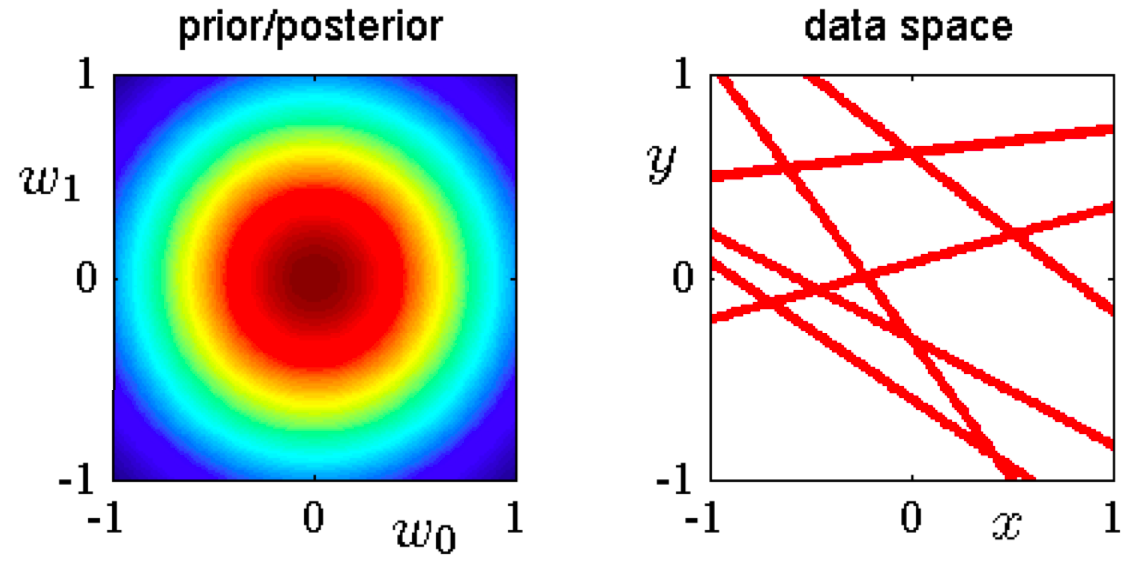
\includegraphics[width=0.6\textwidth]{figures/lin-regression-prior-PRMLFig3-7}
\par\end{center}

\begin{itemize}
\item On right,  $y(x)=\ex\left[y\mid x,w\right]=w_{0}+w_{1}x$, for randomly
chosen $w\sim p(w)=\cn\left(0,\frac{1}{2}I\right)$. 
\end{itemize}
\let\thefootnote\relax\footnotetext{\tiny{Bishop's PRML Fig 3.7}}
\end{frame}


\begin{frame}{Example in 1-Dimension: 1 Observation}
\begin{center}
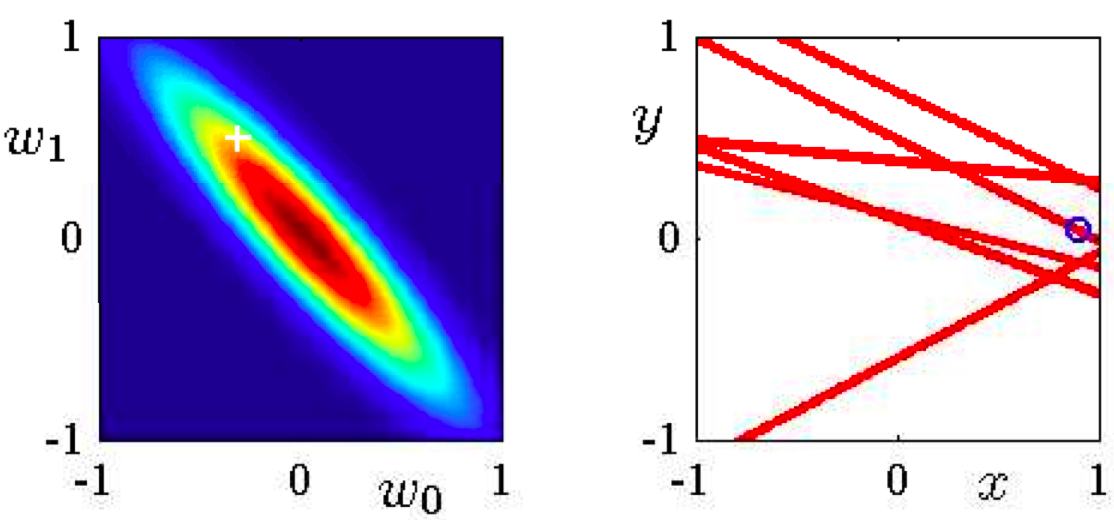
\includegraphics[width=0.6\textwidth]{{figures/lin-regression-prior-PRMLFig3-7.1pt}.png}
\par\end{center}
\begin{itemize}
\item On left: posterior distribution; white cross indicates true parameters
\item On right: 
\begin{itemize}
  \item blue circle indicates the training observation
  \item red lines,  $y(x)=\ex\left[y\mid x,w\right]=w_{0}+w_{1}x$, for randomly
  chosen $w\sim p(w | \cd )$ (posterior)
\end{itemize}
\end{itemize}

\let\thefootnote\relax\footnotetext{\tiny{Bishop's PRML Fig 3.7}}
\end{frame}
%
\begin{frame}{Example in 1-Dimension: 2 and 20 Observations}
\begin{center}
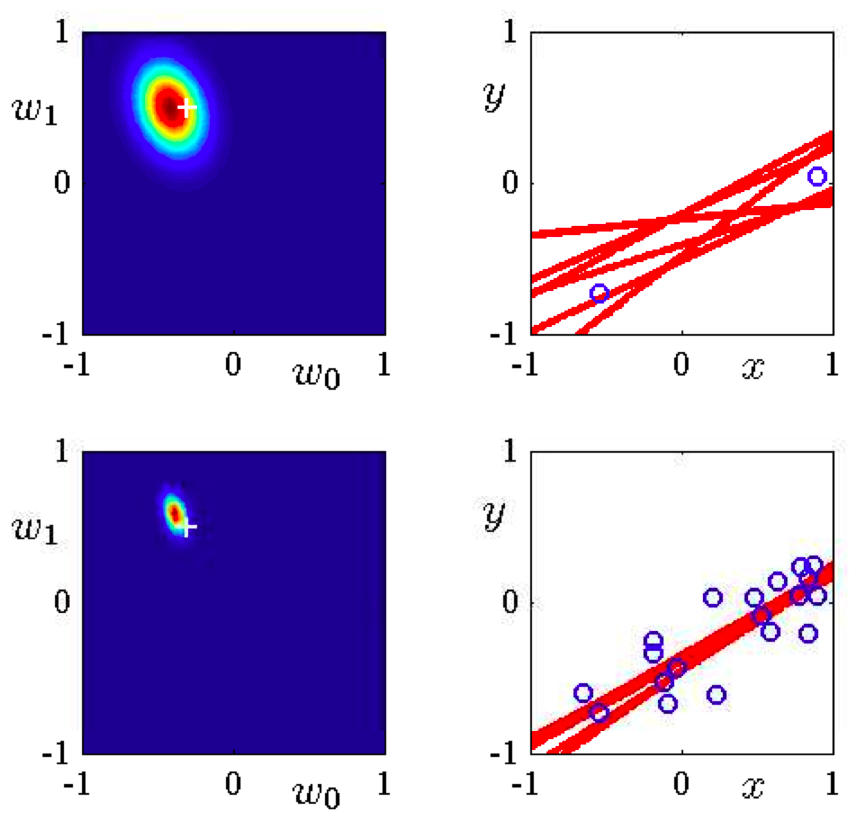
\includegraphics[height=0.7\textheight]{{figures/lin-regression-prior-PRMLFig3-7.2and20pt}.png}
\par\end{center}

\let\thefootnote\relax\footnotetext{\tiny{Bishop's PRML Fig 3.7}}
\end{frame}
%

\section{Gaussian Regression: Closed form}
\begin{frame}{Closed Form for Posterior}
\begin{itemize}
\item Model:
\begin{eqnarray*}
w & \sim & \cn\left(0,\Sigma_{0}\right)\\
\pause y_{i}\mid x,w & \text{i.i.d.} & \cn(w^{T}x_{i},\sigma^{2})
\end{eqnarray*}


\pause{}
\item Design matrix $X$ $\qquad$Response column vector $y$

\pause{}
\item \textbf{Posterior distribution is a Gaussian distribution:
\begin{eqnarray*}
w\mid\cd & \sim & \pause\cn(\mu_{P},\Sigma_{P})\\
\mu_{\text{P}} & = & \left(X^{T}X+\sigma^{2}\Sigma_{0}^{-1}\right)^{-1}X^{T}y\\
\Sigma_{\text{P}} & = & \left(\sigma^{-2}X^{T}X+\Sigma_{0}^{-1}\right)^{-1}
\end{eqnarray*}
}

\pause{}
\item \textbf{Posterior Variance} $\Sigma_{P}$ gives us a natural \textbf{uncertainty
measure.}
\end{itemize}

\end{frame}
%
\begin{frame}{Closed Form for Posterior}
\begin{itemize}
\item \textbf{Posterior distribution is a Gaussian distribution:
\begin{eqnarray*}
w\mid\cd & \sim & \pause\cn(\mu_{P},\Sigma_{P})\\
\mu_{\text{P}} & = & \left(X^{T}X+\sigma^{2}\Sigma_{0}^{-1}\right)^{-1}X^{T}y\\
\Sigma_{\text{P}} & = & \left(\sigma^{-2}X^{T}X+\Sigma_{0}^{-1}\right)^{-1}
\end{eqnarray*}
}

\pause{}
\item If we want point estimates of $w$\textbf{, MAP estimator} and the
\textbf{posterior mean} are given by
\[
\pause\hat{w}=\mu_{P}=\left(X^{T}X+\sigma^{2}\Sigma_{0}^{-1}\right)^{-1}X^{T}y
\]
 

\pause{}
\item For the prior variance $\Sigma_{0}=\frac{\sigma^{2}}{\lambda}I$,
we get
\[
\hat{w}=\mu_{P}=\left(X^{T}X+\lambda I\right)^{-1}X^{T}y,\pause
\]
which is of course the ridge regression solution. 
\end{itemize}
\end{frame}
%
% \begin{comment}
\begin{frame}{Connection the MAP to Ridge Regression}
\begin{itemize}
\item The \textbf{Posterior density }on $w$\textbf{ }for\textbf{ }$\Sigma_{0}=\frac{\sigma^{2}}{\lambda}I$:\textbf{
\begin{eqnarray*}
p(w\mid\cd) & \propto & \underbrace{\exp\left(-\frac{\lambda}{2\sigma^{2}}\|w\|^{2}\right)}_{\text{prior}}\underbrace{\prod_{i=1}^{n}\exp\left(-\frac{(y_{i}-w^{T}x_{i})^{2}}{2\sigma^{2}}\right)}_{\text{likelihood}}
\end{eqnarray*}
}

\pause{}
\item To find the \textbf{MAP}, we minimize the negative log posterior:
\begin{eqnarray*}
\hat{w}_{\text{MAP}} & = & \argmin_{w\in\reals^{d}}\left[-\log p(w\mid\cd)\right]\\
\pause & = & \argmin_{w\in\reals^{d}}\underbrace{\sum_{i=1}^{n}(y_{i}-w^{T}x_{i})^{2}}_{\text{log-likelihood}}+\underbrace{\lambda\|w\|^{2}}_{\text{log-prior}}
\end{eqnarray*}


\pause{}
\item Which is the ridge regression objective.
\end{itemize}
\end{frame}
%
\begin{frame}{Predictive Posterior Distribution}
\begin{itemize}
\item Given a new input point $x_{\text{new}}$, how do we predict $y_{\text{new}}$
?

\pause{}
\item \textbf{Predictive distribution
\begin{eqnarray*}
p(y_{\text{new}}\mid x_{\text{new}},\cd) & = & \pause\int p(y_{\text{new}}\mid x_{\text{new}},w,\cd)p(w\mid\cd)\,dw\\
\pause & = & \int p(y_{\text{new}}\mid x_{\text{new}},w)p(w\mid\cd)\,dw
\end{eqnarray*}
}

\pause{}
\item For Gaussian regression, predictive distribution has closed form.
\end{itemize}
\end{frame}
%
\begin{frame}{Closed Form for Predictive Distribution}
\begin{itemize}
\item \textbf{Model}:
\begin{eqnarray*}
w & \sim & \cn\left(0,\Sigma_{0}\right)\\
\pause y_{i}\mid x,w & \text{i.i.d.} & \cn(w^{T}x_{i},\sigma^{2})
\end{eqnarray*}


\pause{ }
\item \textbf{Predictive Distribution}
\begin{eqnarray*}
p(y_{\text{new}}\mid x_{\text{new}},\cd) & = & \int p(y_{\text{new}\text{ }}\mid x_{\text{new}},w)p(w\mid\cd)\,dw.
\end{eqnarray*}

\begin{itemize}
\item Averages over prediction for each $w$, weighted by posterior distribution.

\pause{ }
\end{itemize}
\item \textbf{Closed form:}
\begin{eqnarray*}
y_{\text{new}}\mid x_{\text{new}},\cd & \sim & \cn\left(\eta_{\text{new}}\,,\,\sigma_{\text{new}}^{2}\right)\\
\pause\eta_{\text{new}} & = & \mu_{\text{P}}^{T}x_{\text{new}}\\
\pause\sigma_{\text{new}}^{2} & = & \underbrace{x_{\text{new}}^{T}\Sigma_{\text{P}}x_{\text{new}}}_{\text{from variance in }w}+\underbrace{\sigma^{2}}_{\text{inherent variance in }y}
\end{eqnarray*}
\end{itemize}
\end{frame}

\begin{frame}{Bayesian Regression Provides Uncertainty Estimates}
\begin{itemize}
\item With predictive distributions, we can give mean prediction with error
bands:
\end{itemize}
\begin{center}
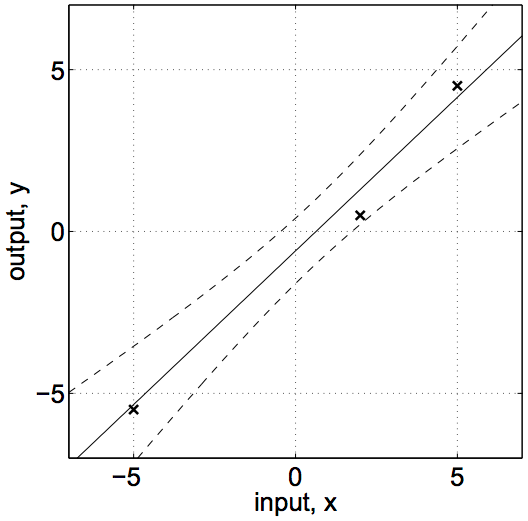
\includegraphics[height=0.7\textheight]{figures/predictiveDistWithErrorBands}
\par\end{center}

\let\thefootnote\relax\footnotetext{\tiny{Rasmussen and Williams' \emph{Gaussian Processes for Machine Learning}, Fig.2.1(b) }}
\end{frame}
% \end{comment}


\section{Overview}
\begin{frame}
{Motivation}
\begin{itemize}
\item So far, most algorithms we've learned are designed for binary classification.
  \begin{itemize}
  \item Sentiment analysis (positive vs. negative)
  \item Spam filter (spam vs. non-spam)
  \end{itemize}
\note[item]{Which ones we've learned can handle more than 2 classes? Multinomial logistic regression, naive Bayes. Next, trees and random forests.}
\pause
\item Many real-world problems have more than two classes.
\begin{itemize}
  \item Document classification (over 10 classes)
  \item Object recognition (over 20k classes)
  \item Face recognition (millions of classes)
\end{itemize}
\note[item]{Examples? Text classification, object recognition (ImageNet has more than 20k classes).}
\pause
\item<2-> What are some potential issues when we have a large number of classes?
\begin{itemize}
  \item Computation cost
  \item Class imbalance
  \item Different cost of errors
\end{itemize}
\note<2->[item]{Class imbalance, computation cost for both training and testing, different cost of errors etc.}
\end{itemize}
\end{frame}

\begin{frame}
{Today's lecture}
\begin{itemize}
\item How to \emph{reduce} multiclass classification to binary classification?
\begin{itemize}
  \item We can think of binary classifier or linear regression as a black box. Naive ways:
  \item E.g. multiple binary classifiers produce a binary code for each class (000, 001, 010)
  \item E.g. a linear regression produces a numerical value for each class (1.0, 2.0, 3.0)
\end{itemize}
\pause
\note[item]{Think of binary classification or linear regression as black-box predictors and start from there.}
\item How do we \emph{generalize} binary classification algorithm to the multiclass setting?
\begin{itemize}
  \item We also need to think about the loss function.
\end{itemize}
\pause
% \note[item]{What needs to be changed here? The loss function.}
\item Example of very large output space: structured prediction.
\begin{itemize}
  \item Multi-class: Mutually exclusive class structure.
  \item Text: Temporal relational structure.
\end{itemize}
\end{itemize}
\end{frame}

\section{Reduction to Binary Classification}
\subsection{Recap: OvA and AvA}
\begin{frame}{One-vs-All / One-vs-Rest}
\begin{description}
    \setlength\itemsep{10pt}
\item<+->[Setting]
\begin{itemize}
\item Input space: $\cx$
\item Output space: $\cy=\left\{ 1,\ldots,k\right\} $
\end{itemize}

\item<+->[Training]
\begin{itemize}
\item Train $k$ binary classifiers, one for each class:
$h_{1},\ldots,h_{k}:\cx\to\reals$.
\item Classifier $h_i$ distinguishes class $i$ (+1) from the rest (-1).
\end{itemize}

\item<+->[Prediction]
\begin{itemize}
\item Majority vote:
\[
h(x)=\argmax_{i\in\left\{ 1,\ldots,k\right\} }h_{i}(x)
\]
\item Ties can be broken arbitrarily.
\end{itemize}
\end{description}
\end{frame}
%

\begin{frame}
{OvA: 3-class example (linear classifier)}
\begin{columns}
\begin{column}{0.4\textwidth}
\begin{simpleblock}<1->
{Consider a dataset with three classes:}
\begin{figure}
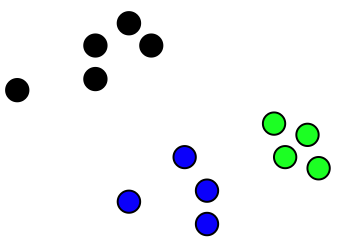
\includegraphics[height=0.25\textheight]{figures/three-class}
\end{figure}
\end{simpleblock}
\end{column}
\begin{column}{0.6\textwidth}
\onslide<3->{
\textbf{Assumption}: each class is linearly separable from the rest.\\
Ideal case: only target class has positive score.
}
\end{column}
\end{columns}

\begin{simpleblock}<2->
{Train OvA classifiers:}
\begin{figure}
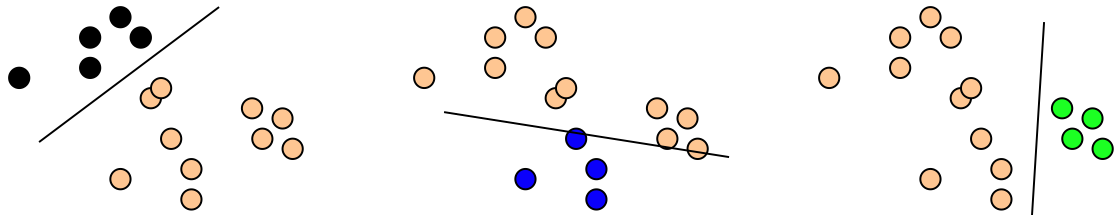
\includegraphics[height=0.25\textheight]{figures/three-class-ova}
\end{figure}
\end{simpleblock}
\note<3->{What's a failure case for OvA?}
\end{frame}

\begin{frame}
{OvA: 4-class non linearly separable example}
\begin{columns}
\begin{column}{0.4\textwidth}
Consider a dataset with four classes:
\begin{figure}
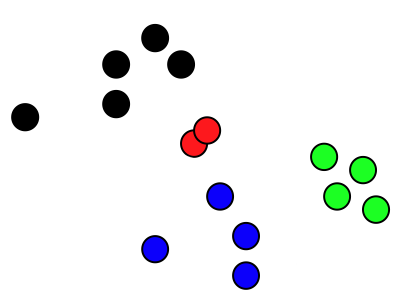
\includegraphics[height=0.25\textheight]{figures/four-class}
\end{figure}
\end{column}
\begin{column}{0.6\textwidth}
\onslide<2->{
Cannot separate \textcolor{red}{red} points from the rest.\\
Which classes might have low accuracy?
}
\note<2->[item]{Blue and green because they are getting positive score from the red classifier.}
\end{column}
\end{columns}

Train OvA classifiers:
\begin{figure}
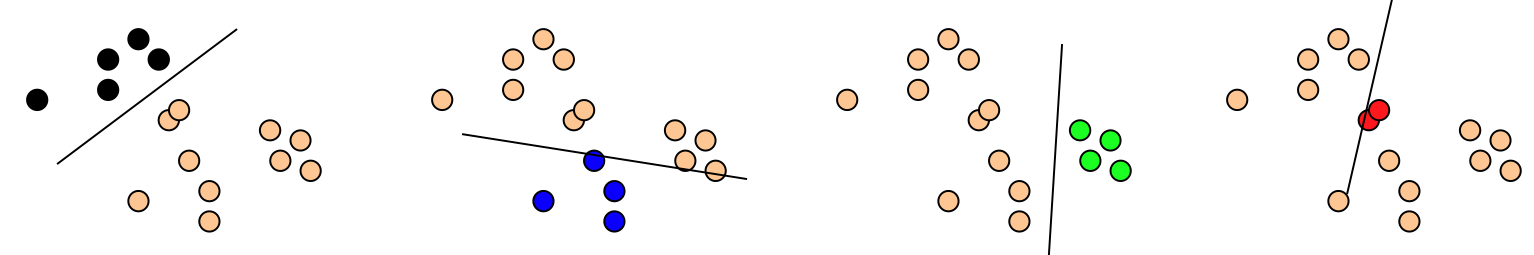
\includegraphics[height=0.25\textheight]{figures/four-class-ova}
\end{figure}
\note<2->[item]{How can we fix this? Note that optimal linear classifiers exist in this example.}
\end{frame}

\begin{frame}
{All vs All / One vs One / All pairs}
\begin{description}
    \setlength\itemsep{10pt}
\item<1->[Setting]
\begin{itemize}
    \setlength\itemsep{2pt}
\item Input space: $\cx$
\item Output space: $\cy=\left\{ 1,\ldots,k\right\} $
\end{itemize}
\note<1>[item]{How many classifiers do we need to train?}

\item<2->[Training]
\begin{itemize}
    \setlength\itemsep{2pt}
\item Train $k \choose 2$ binary classifiers, one for each pair:
$h_{ij}:\cx\to\reals$ $\text{for } i\in [1,k] \text{ and } j\in [i+1, k]$.
\item Classifier $h_{ij}$ distinguishes class $i$ (+1) from class $j$ (-1).
\end{itemize}

\item<3->[Prediction]
\begin{itemize}
    \setlength\itemsep{2pt}
\item Majority vote (each class gets $k-1$ votes)
\[
h(x)=\argmax_{i\in\left\{ 1,\ldots,k\right\} } \sum_{j\neq i}
\underbrace{h_{ij}(x)\1\pc{i<j}}_{\text{class $i$ is +1}} 
- \underbrace{h_{ji}(x)\1\pc{j<i}}_{\text{class $i$ is -1}}
\]
\note<3->[item]{Majority vote: Class $i$ gets a vote each time it is predicted.}
\item Tournament
\note<3->[item]{Tournament: start with random pairs, only winners continue.}
\item Ties can be broken arbitrarily.
\end{itemize}
\end{description}
\end{frame}

\begin{frame}
{AvA: four-class example}
\begin{columns}
\begin{column}{0.4\textwidth}
Consider a dataset with four classes:
\begin{figure}
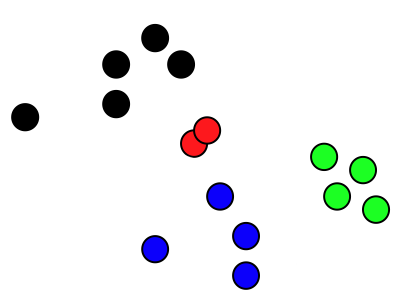
\includegraphics[height=0.25\textheight]{figures/four-class}
\end{figure}
\end{column}
\begin{column}{0.6\textwidth}
\onslide<2->{
\textbf{Assumption}: each pair of classes are linearly separable.\\
More expressive than OvA.
}
\end{column}
\end{columns}

What's the decision region for the red class?
\begin{figure}
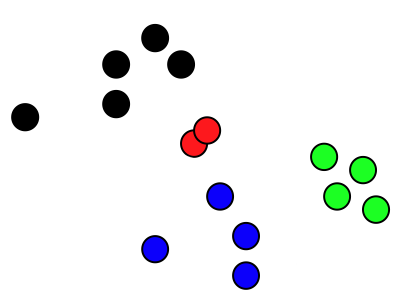
\includegraphics[height=0.3\textheight]{figures/four-class}
\end{figure}
\note<1>[item]{Draw lines separating red from each other classes. The intersection of the three regions get 3 votes (max).}
\end{frame}

\begin{frame}
{OvA vs AvA}
\begin{table}
\begin{tabular}{llcc}

\toprule
& & OvA & AvA \\
\midrule
\multirow{2}{*}{computation} & train & $O(k \onslide<2->{B_{\text{train}}(n)})$ & $O(k^2\onslide<2->{B_{\text{train}}(n/k)})$ \\
                                     &  test & $O(k\onslide<2->{B_{\text{test}}})$ & $O(k^2 \onslide<2->{B_{\text{test}}})$ \\
       \midrule

\pause
\multirow{3}{*}{challenges}  \pause  & train & class imbalance & small training set \\
                                                   & \multirow{2}{*}{test} & \multicolumn{2}{c}{calibration / scale} \\
                                                    &         &  \multicolumn{2}{c}{tie breaking} \\
\bottomrule

\end{tabular}
\end{table}
Lack theoretical justification but simple to implement and works well in practice (when \# classes is small).

%\think{Question}: When would you prefer AvA / OvA? 
%\note{If you're using SVM, would you prefer AvA or OvA to save computation?
%Dual form would prefer AvA. When number of examples much larger than feature dimensions, dual is more expensive.}
\end{frame}

\subsection{Error correcting output codes}

\begin{frame}
{Code word for labels}
Using the reduction approach, can you train fewer than $k$ binary classifiers?
\pause

\textbf{Key idea}: Encode labels as binary codes and predict the code bits directly.
\pause

OvA encoding:
\begin{table}
\begin{tabular}{|c|c|c|c|c|}
\hline
class & $h_1$ & $h_2$ & $h_3$ & $h_4$ \\
\hline
1 & 1 & 0 & 0 & 0 \\
\hline
2 & 0 & 1 & 0 & 0\\
\hline
3 & 0 & 0 & 1 & 0\\
\hline
4 & 0 & 0 & 0 & 1\\
\hline
\end{tabular}
\end{table}
\pause

OvA uses $k$ bits to encode each label, what's the minimal number of bits you can use?
\end{frame}

\begin{frame}
{Error correcting output codes (ECOC)}
\begin{columns}
\begin{column}{0.4\textwidth}
Example: 8 classes, 6-bit code
\begin{table}
\begin{tabular}{|c|c|c|c|c|c|c|}
\hline
class & $h_1$ & $h_2$ & $h_3$ & $h_4$ &  $h_5$ & $h_6$\\
\hline
1 & 0 & 0 & 0 & 1 & 0 & 0 \\
\hline
2 & 1 & 0 & 0 & 0 & 0 & 0 \\
\hline
\rowcolor{red!20}
3 & 0 & 1 & 1 & 0 & 1 & 0\\
\hline
4 & 1 & 1 & 0 & 0 & 0 & 0 \\
\hline
5 & 1 & 1 & 0 & 0 & 1 & 0 \\
\hline
6 & 0 & 0 & 1 & 1 & 0 & 1 \\
\hline
7 & 0 & 0 & 1 & 0 & 0 & 0 \\
\hline
8 & 0 & 1 & 0 & 1 & 0 & 0 \\
\hline
\end{tabular}
\end{table}
\end{column}
%
\begin{column}{0.6\textwidth}
\begin{description}
\item<1->[Training]
Binary classifier $h_i$: 
\begin{itemize}
\item +1: classes whose $i$-th bit is 1
\item -1: classes whose $i$-th bit is 0
\end{itemize}
\item<2->[Prediction]
Closest label in terms of Hamming distance.
\begin{table}
\begin{tabular}{{|c|c|c|c|c|c|}}
\hline
$h_1$ & $h_2$ & $h_3$ & $h_4$ &  $h_5$ & $h_6$\\
\hline
0 & 1 & 1 & 0 & 1 & 1 \\
\hline
\end{tabular}
\end{table}
\item<3->[Code design]
Want good binary classifiers.
\note<3->[item]{Random or depending on domain knowledge}
\end{description}
\end{column}
\end{columns}
\end{frame}

\begin{frame}
{Error correcting output codes: summary}
\begin{itemize}
\item Computationally more efficient than OvA (a special case of ECOC). Better for large $k$.
\item Why not use the minimal number of bits ($\log_2k$)?
\pause
\begin{itemize}
\item If the minimum Hamming distance between any pair of code word is $d$, then it can correct $\left \lfloor \frac{d-1}{2} \right \rfloor$ errors.
\item In plain words, if rows are far from each other, ECOC is robust to errors.
\end{itemize}
\pause
\item Trade-off between code distance and binary classification performance.
\note<2>[item]{Larger distance -> more binary problems -> more likely to have hard binary problems.}
\item Nice theoretical results \href{http://www.jmlr.org/papers/volume1/allwein00a/allwein00a.pdf}{[Allwein et al., 2000]} (also incoporates AvA).
\end{itemize}
\end{frame}

\begin{frame}
{Review}
Reduction-based approaches:
\begin{itemize}
\item Reducing multiclass classification to binary classification: OvA, AvA%, ECOC.
\item Key is to design \textcolor{Green}{``natural'' binary classification} problems without large \textcolor{red}{computation} cost.
\end{itemize}
\pause

But,
\begin{itemize}
\item Unclear how to generalize to extremely large \# of classes.
\item ImageNet: >20k labels; Wikipedia: >1M categories.
\end{itemize}

Next,
generalize previous algorithms to multiclass settings.
\note<2->[item]{What needs to be changed? The loss function.}
\end{frame}

\section{Multiclass Loss}

\begin{frame}{Binary Logistic Regression}
\begin{itemize}
\item Given an input x, we would like to output a classification between (0,1).
\begin{align}
f(x) = sigmoid(z) = \frac{1}{1+ \exp(-z)}= \frac{1}{1 + \exp(- w^\top x-b)}.
\end{align}
\pause
\item The other class is represented in $1 - f(x)$:
\begin{align}
1 - f(x) &= \frac{\exp(-w^\top x-b)}{1 + \exp(-w^\top x-b)} = \frac{1}{1+ \exp(w^\top x +b)} = sigmoid(-z).
\end{align}
\pause
\item Another way to view: one class has $(+w, +b)$ and the other class has $(-w, -b)$.
\end{itemize}
\end{frame}

\begin{frame}{Multi-class Logistic Regression}
\begin{itemize}
  \item Now what if we have one $w_c$ for each class $c$?

  \pause
 \begin{align}
  f_c(x) = \frac{\exp(w_c^\top x) + b_c}{\sum_c \exp(w_c^\top x + b_c)}
  \end{align}
  \item Also called ``softmax'' in neural networks.

  \pause
  \item Loss function:
  $L = \sum_i -y_c^{(i)} \log f_c(x^{(i)})$

  \pause
  \item Gradient: $\frac{\partial L}{\partial z} = f - y$. Recall: MSE loss.
\end{itemize}
\end{frame}

\begin{frame}
{Comparison to OvA}
\begin{itemize}
\item \textbf{Base Hypothesis Space}: $\ch=\left\{ h:\cx\to\reals\right\} $
(\textcolor{blue}{score functions}).
\item \textbf{Multiclass Hypothesis Space} (for $k$ classes): 
\[
\cf=\left\{ x\mapsto\argmax_{i}h_{i}(x)\mid h_{1},\ldots,h_{k}\in\ch\right\} 
\]

\pause{}
\item Intuitively, $h_{i}(x)$ scores how likely $x$ is to be from class $i$.

\item OvA objective: $h_i(x) > 0$ for $x$ with label $i$ and
$h_i(x) < 0$ for $x$ with all other labels.

\pause
\item At test time, to predict $(x, i)$ correctly we only need
\begin{align}
h_i(x) > h_j(x) \qquad \forall j \neq i .
\end{align}
\end{itemize}
\end{frame}

\begin{frame}
{Multiclass Perceptron}
\begin{itemize}
\item Base linear predictors: $h_i(x) = w_i^Tx$ ($w\in \bR^d$).
\pause
\item Multiclass perceptron:
\begin{algorithm}[H]
  Given a multiclass dataset $\sD=\pc{(x, y)}$\;
  Initialize $w\leftarrow 0$\;
  \For{$\text{iter} = 1,2,\ldots,T$}{
  \For{$(x,y) \in \sD$}
  {
    $\hat{y} = \argmax_{y'\in\sY} w_{y'}^Tx$\;
    \If(\tcp*[h]{We've made a mistake}){$\hat{y} \neq y$}{ 
    $w_y \leftarrow w_y + x$ \tcp*[l]{Move the target-class scorer towards $x$}
    $w_{\hat{y}} \leftarrow w_{\hat{y}} - x$ \tcp*[l]{Move the wrong-class scorer away from $x$}
    }
    }
    }
\end{algorithm}
\end{itemize}
\end{frame}

% \begin{frame}{Linear Binary Classifier Review}

% \begin{itemize}
% \item Input Space: $\cx=\reals^{d}$
% \item Output Space: $\cy=\left\{ -1,1\right\} $ 
% \end{itemize}

% \begin{itemize}
% \item Linear classifier score function:
% \begin{eqnarray*}
% f(x) & = & \left\langle w,x\right\rangle =w^{T}x
% \end{eqnarray*}

% \pause{}
% \item Final classification prediction: $\sign\left(f(x)\right)$
% \item Geometrically, when are $\sign\left(f(x)\right)=+1$ and $\sign\left(f(x)\right)=-1$? 
% \end{itemize}
% \end{frame}
% %
% \begin{frame}{Linear Binary Classifier Review}

% \begin{center}
% 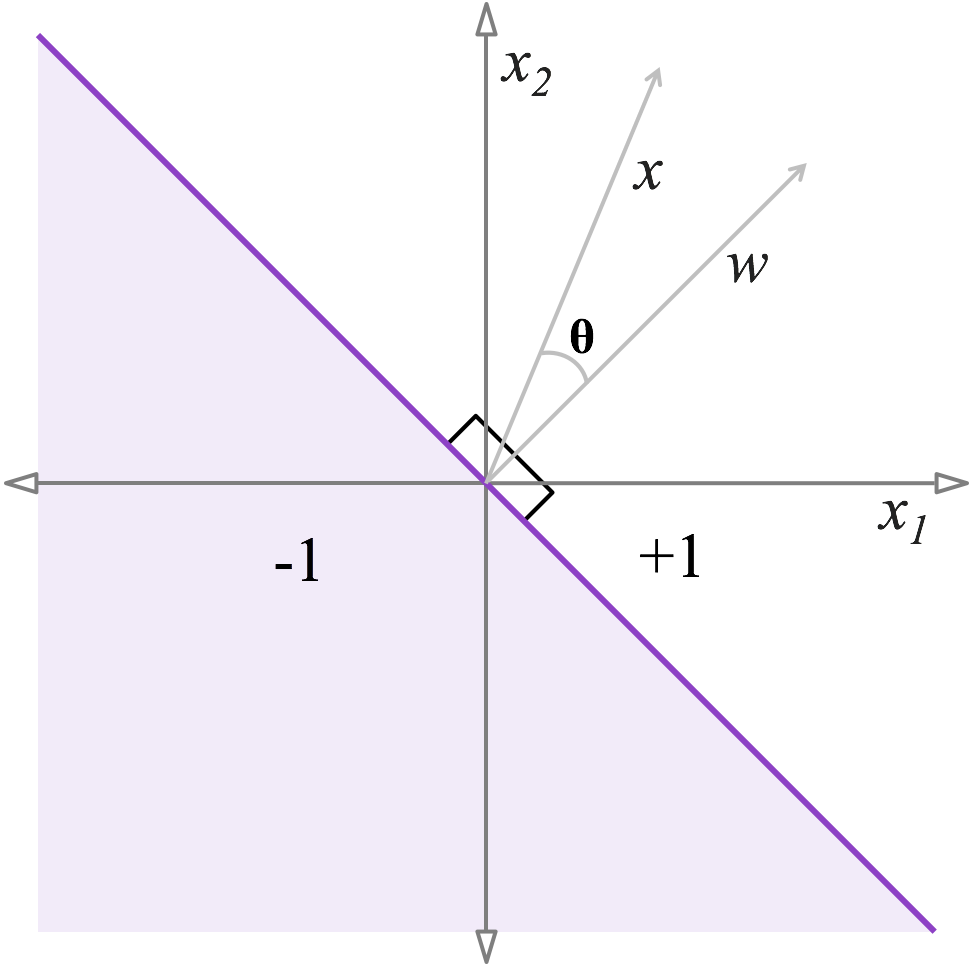
\includegraphics[height=0.45\textheight]{figures/linear-separator}
% \par\end{center}

% Suppose $\|w\|>0$ and $\|x\|>0$: 
% \begin{eqnarray*}
% f(x) & = & \left\langle w,x\right\rangle =\|w\|\|x\|\cos\theta\\
% f(x)>0 & \iff & \cos\theta>0 \iff\theta\in\left(-90^{\circ},90^{\circ}\right)\\
% f(x)<0 & \iff & \cos\theta<0 \iff\theta\not\in[-90^{\circ},90^{\circ}]
% \end{eqnarray*}

% \end{frame}

\begin{frame}
{Rewrite the scoring function}
\begin{itemize}
\item Remember that we want to scale to very large \# of classes and
reuse algorithms and analysis for binary classification
\begin{itemize}
\item $\implies$ a \textcolor{blue}{single weight vector} is desired
\end{itemize}

\item How to rewrite the equation such that we have one $w$ instead of $k$?
\pause
\begin{align}
w_i^Tx &= w^T\psi(x, i) \\
h_i(x) &= h(x, i)
\end{align}
\begin{itemize}
\item Encode labels in the feature space.
\item Score for each label $\rightarrow$ score for the ``\emph{compatibility}'' of a label and an input.
\end{itemize}
\end{itemize}
\end{frame}

\begin{frame}{The Multivector Construction}
How to construct the feature map $\psi$?
\pause
\begin{itemize}
\item What if we stack $w_{i}$'s together (\eg $x\in \bR^2, \sY = \pc{1,2,3}$)
\[
w=\left(\underbrace{-\frac{\sqrt{2}}{2},\frac{\sqrt{2}}{2}}_{w_{1}},\underbrace{0,1}_{w_{2}},\underbrace{\frac{\sqrt{2}}{2},\frac{\sqrt{2}}{2}}_{w_{3}}\right)
\]
\end{itemize}
\pause
\begin{itemize}
\item And then do the following: $\Psi:\reals^{2}\times\left\{ 1,2,3\right\} \to\reals^{6}$
defined by
\begin{eqnarray*}
\Psi(x,1) & := & \left(x_{1},x_{2},0,0,0,0\right)\\
\Psi(x,2) & := & \left(0,0,x_{1},x_{2},0,0\right)\\
\Psi(x,3) & := & \left(0,0,0,0,x_{1},x_{2}\right)
\end{eqnarray*}
\pause
\item Then $\left\langle w,\Psi(x,y)\right\rangle =\left\langle w_{y},x\right\rangle $,
which is what we want. 
\end{itemize}
\end{frame}


\begin{frame}
{Rewrite multiclass perceptron}
Multiclass perceptron using the multivector construction.

\begin{algorithm}[H]
  Given a multiclass dataset $\sD=\pc{(x, y)}$\;
  Initialize $w\leftarrow 0$\;
  \For{$\text{iter} = 1,2,\ldots,T$}{
  \For{$(x,y) \in \sD$}
  {
    $\hat{y} = \argmax_{y'\in \sY} w^T\psi(x, y')$ \tcp*[l]{Equivalent to $\argmax_{y'\in\sY} w_{y'}^Tx$}
    \If(\tcp*[h]{We've made a mistake}){$\hat{y} \neq y$}{ 
    $w \leftarrow w + \psi(x, y)$ \tcp*[l]{Move the scorer towards $\psi(x, y)$}
    $w \leftarrow w - \psi(x, \hat{y})$ \tcp*[l]{Move the scorer away from $\psi(x, \hat{y})$}
    }
    }
    }
\end{algorithm}
\pause
\textcolor{Green}{Exercise}: What is the base binary classification problem in multiclass perceptron?
\note{$w^T(\phi(x,i)-\phi(x,j)) > 0$.}
\end{frame}

\begin{frame}
{Features}
Toy multiclass example: Part-of-speech classification
\begin{itemize}
\item $\cx=\left\{ \mbox{All possible words}\right\} $
\item $\cy=\left\{ \mbox{NOUN,VERB,ADJECTIVE,\ldots}\right\} $.
\note<1>{What are useful features?}
\pause{}
\item Features of $x\in\cx$: $\mbox{[The word itself], ENDS\_IN\_ly, ENDS\_IN\_ness, ...}$
\end{itemize}

How to construct the feature vector?
\begin{itemize}
\item Multivector construction: $w\in \bR^{d\times k}$---\textcolor{red}{doesn't scale}.
\pause
\item Directly design features for each class.
\begin{align}
\Psi(x,y)=\left(\psi_{1}(x,y),\psi_{2}(x,y),\psi_{3}(x,y),\ldots,\psi_{d}(x,y)\right)
\end{align}
\begin{itemize}
\item Size can be bounded by $d$.
\end{itemize}
\end{itemize}
\end{frame}

\begin{frame}
{Features}
Sample training data:
\begin{center}
\texttt{
The boy grabbed the apple and ran away quickly .
}
\end{center}
\pause

Feature:
\begin{eqnarray*}
\psi_{1}(x,y) & = & \ind{x=\mbox{apple AND }y=\mbox{NOUN}}\\
\psi_{2}(x,y) & = & \ind{x=\mbox{run AND }y=\mbox{NOUN}}\\
\psi_{3}(x,y) & = & \ind{x=\mbox{run AND }y=\mbox{VERB}}\\
\psi_{4}(x,y) & = & \ind{x\mbox{ ENDS\_IN\_ly AND \ensuremath{y=}ADVERB}}\\
\ldots
\end{eqnarray*}
\pause
\vspace{-2em}
\begin{itemize}[<+->]
\item E.g., $\Psi(x=\text{run},y=\text{NOUN})=\left(0,1,0,0,\ldots\right)$
\item After training, what's $w_{1},w_{2},w_{3},w_{4}$?
\item \textcolor{blue}{No need to include features unseen in training data}.
\end{itemize}

\end{frame}

\begin{frame}
{Feature templates: implementation}
\begin{itemize}
\item Flexible, \eg neighboring words, suffix/prefix.
\item ``Read off'' features from the training data.
\item Often sparse---efficient in practice, \eg NLP problems.
\item Can use a hash function: template $\rightarrow \pc{1, 2, \ldots, d}$.
\end{itemize}
\end{frame}

\begin{frame}
{Review}
Ingredients in multiclass classification:
\begin{itemize}
\item Scoring functions for each class (similar to ranking).
\item Represent labels in the input space $\implies$ single weight vector.
\end{itemize}
\pause

We've seen
\begin{itemize}
\item How to generalize the perceptron algorithm to multiclass setting.
\item Very simple idea. Was popular in NLP for structured prediction (\eg tagging, parsing).
\end{itemize}
\pause

Next,
\begin{itemize}
\item How to generalize SVM to the multiclass setting.
\item \think{Concept check}: Why might one prefer SVM / perceptron?
\note{Uniqueness of solution, online learning / efficiency, inductive bias (margin)}
\end{itemize}
\end{frame}

%================================== 


\subsection{Linear Multiclass SVM}
\subsubsection{Formulation through constraints on margin}

\begin{frame}{Margin for Multiclass}
\begin{description}
\item<1->[Binary]
\begin{itemize}
\item Margin for $(\xn, \yn)$:
\begin{align}
\yn w^T\xn
\end{align}
\item Want margin to be large and positive ($w^T\xn$ has same sign as $\yn$)
\end{itemize}

\item<2->[Multiclass]
\begin{itemize}
\item Class-specific margin for $(\xn, \yn)$:
\begin{align}
h(\xn,\yn)-h(\xn,y).
\end{align}
\item Difference between scores of the correct class and each other class
\item Want margin to be large and positive for all $y\neq \yn$. 
\end{itemize}
\end{description}
\end{frame}
%

\begin{frame}
{Multiclass SVM: separable case}
\begin{description}
\item<1->[Binary] 
\begin{align}
\min_w \quad & \frac{1}{2}\|w\|^2 \\
\text{s.t.} \quad& \underbrace{\yn w^T\xn}_{\text{margin}} \geq 1 \quad \forall (\xn, \yn) \in \sD
\end{align}

\item<2->[Multiclass] As in the binary case, take 1 as our target margin.
\begin{align}
m_{n,y}(w)&\eqdef \underbrace{\left\langle w,\Psi(\xn,\yn)\right\rangle}_{\text{score of correct class}}
- \underbrace{\left\langle w,\Psi(\xn,y)\right\rangle}_{\text{score of other class}} \\
\min_w \quad & \frac{1}{2}\|w\|^2 \\
\text{s.t.} \quad& m_{n,y}(w) \geq 1 \quad
\forall (\xn, \yn) \in \sD,\, y\neq \yn
\end{align}

\end{description}
\onslide<3->{
\think{Exercise}: write the objective for the non-separable case
}
\note<3->{Next, let's think about how to write the objective using hinge loss.}
\end{frame}

\subsubsection{Formulation through hinge loss}
\begin{frame}
{Recap: hingle loss for binary classification}
\begin{itemize}
\item Hinge loss: a convex upperbound on the 0-1 loss
\begin{align}
\ell_{\text{hinge}}(y, \hat{y}) = \max(0, 1 -  yh(x))
\end{align}
\begin{figure}
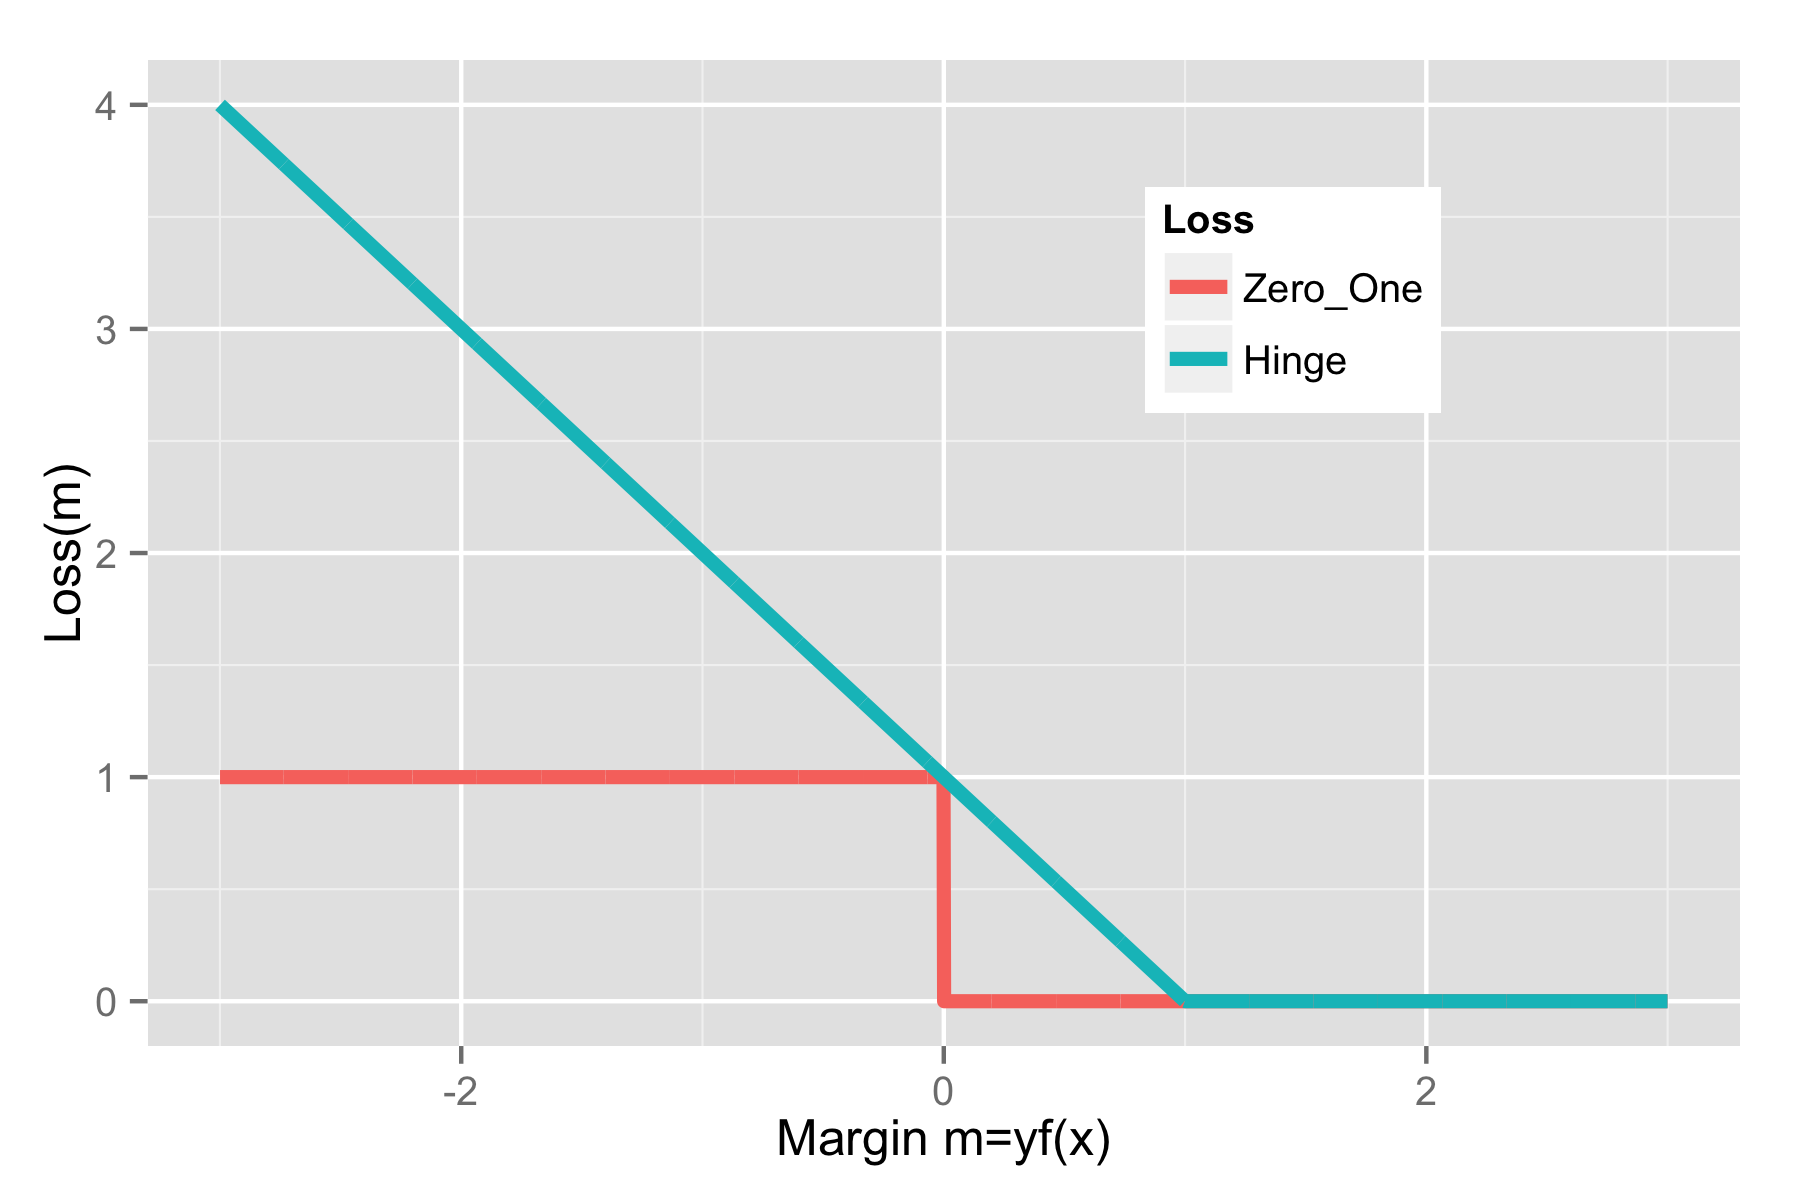
\includegraphics[height=0.5\textheight]{{figures/loss.Zero_One.Hinge}.png}
\end{figure}
\end{itemize}
\end{frame}

\begin{frame}
{Generalized hinge loss}
\begin{itemize}[<+->]
\item What's the zero-one loss for multiclass classification?
\begin{align}
\onslide<+->{\Delta(y, y') = \1\pc{y\neq y'}}
\end{align}
\item In general, can also have different cost for each class.

\item Upper bound on $\Delta(y, y')$.
\begin{align}
\hat{y} &\eqdef \argmax_{y'\in\sY} \left\langle w, \Psi(x, y') \right\rangle \\
\onslide<+->{
\implies & \left\langle w, \Psi(x, y) \right\rangle \leq
\left\langle w, \Psi(x, \hat{y}) \right\rangle \\
}
\onslide<+->{
\implies & \Delta(y, \hat{y}) \leq \Delta(y, \hat{y}) -
\left\langle w, \p{\Psi(x, {y}) - \Psi(x, \hat{y}}) \right\rangle
&& \text{When are they equal?}
}
\end{align}

\item Generalized hinge loss:
\begin{align}
\ell_\text{hinge}(y, x, w) \eqdef
\max_{y'\in\sY}\p{
\Delta(y, {y'}) -
\left\langle w, \p{\Psi(x, {y}) - \Psi(x, {y'}}) \right\rangle
}
\end{align}
% \note<+->{When $y'=y$, $\ell_{\text{hinge}}=0$.}
\end{itemize}
\end{frame}

\begin{frame}{Multiclass SVM with Hinge Loss}
 
\begin{itemize}
\item Recall the hinge loss formulation for binary SVM (without the bias term):
\[
\min_{w\in\reals^{d}}\frac{1}{2}||w||^{2}+C\sum_{n=1}^{N}\max\left(0,1-\underbrace{\yn w^{T}\xn}_{\text{margin}}\right).
\]

\pause{}
\item The multiclass objective: 
\[
\min_{w\in\reals^{d}}\frac{1}{2}||w||^{2}+
C\sum_{n=1}^{N}\max_{y'\in\sY} \p{
\Delta(y, {y'}) -
\underbrace{
\left\langle w, \p{\Psi(x, {y}) - \Psi(x, {y'}}) \right\rangle
}_{\text{margin}}
}
\]

\begin{itemize}
\item $\Delta(y, y')$ as \textcolor{blue}{target margin} for each class.
\item If margin $m_{n, y'}(w)$ meets or exceeds its target $\Delta(\yn,y')$
$\forall y\in \sY$, then no loss on example $n$. 
\note<2->{If exceeds margin, loss is negative, which must be smaller than loss of the true class, which is zero.}
\end{itemize}
\end{itemize}
\end{frame}
%

\subsection{Is This Worth The Hassle Compared to One-vs-All?}
\begin{frame}{Recap: What Have We Got?}
\begin{itemize}
\item Problem: Multiclass classification $\cy=\left\{ 1,\ldots,k\right\} $
\end{itemize}

\pause{}
\begin{itemize}
\item Solution 1: One-vs-All


\begin{itemize}
\item Train $k$ models: $h_{1}(x),\ldots,h_{k}(x):\cx\to\reals$.


\item Predict with $\argmax_{y\in\cy}h_{y}(x)$.


\item Gave simple example where this fails for linear classifiers
\end{itemize}
\end{itemize}

\pause{}
\begin{itemize}
\item Solution 2: Multiclass loss


\begin{itemize}
\item Train one model: $h(x,y):\cx\times\cy\to\reals$.


\item Prediction involves solving $\argmax_{y\in\cy}h(x,y)$.
\end{itemize}
\end{itemize}
\end{frame}
%
\begin{frame}{Does it work better in practice?}
\begin{itemize}
\item Paper by Rifkin \& Klautau: ``\href{http://www.jmlr.org/papers/v5/rifkin04a.html}{In Defense of One-Vs-All Classification}''
(2004)
\begin{itemize}
\item Extensive experiments, carefully done 
\begin{itemize}
\item albeit on relatively small UCI datasets
\end{itemize}
\end{itemize}


\begin{itemize}
\item Suggests one-vs-all works just as well in practice
\begin{itemize}
\item (or at least, the advantages claimed by earlier papers for multiclass
methods were not compelling)
\end{itemize}
\end{itemize}
\end{itemize}

\pause
\begin{itemize}
\item Compared 
\begin{itemize}
\item many multiclass frameworks (including the one we discuss)
\item one-vs-all for SVMs with RBF kernel
\item one-vs-all for square loss with RBF kernel (for classification!) 
\end{itemize}
\end{itemize}


\begin{itemize}
\item All performed roughly the same
\end{itemize}
\end{frame}
%
\begin{frame}{Why Are We Bothering with Multiclass?}
\begin{itemize}
\item The framework we have developed for multiclass
\begin{itemize}
\item compatibility features / scoring functions
\item multiclass margin
\item target margin / multiclass loss
\end{itemize}
\end{itemize}

\pause{}
\begin{itemize}
\item Generalizes to situations where \textcolor{blue}{$k$ is very large} and one-vs-all
is intractable.
\end{itemize}

\pause{}
\begin{itemize}
\item Key idea is that we can \textcolor{blue}{generalize across outputs $y$ by using features
of $y$}.
\end{itemize}
\end{frame}

\section{Introduction to Structured Prediction}
\begin{frame}{Example: Part-of-speech (POS) Tagging}

\begin{itemize}
\item Given a sentence, give a part of speech tag for each word:
\end{itemize}
\begin{center}
\begin{tabular}{|c|c|c|c|c|}
\hline 
$x$ & $\underbrace{\mbox{[START]}}_{x_{0}}$ & $\underbrace{\mbox{He}}_{x_{1}}$ & $\underbrace{\mbox{eats}}_{x_{2}}$ & $\underbrace{\mbox{apples}}_{x_{3}}$\tabularnewline
\hline 
$y$ & $\underbrace{\mbox{[START]}}_{y_{0}}$ & $\underbrace{\mbox{Pronoun}}_{y_{1}}$ & $\underbrace{\mbox{Verb}}_{y_{2}}$ & $\underbrace{\mbox{Noun}}_{y_{3}}$\tabularnewline
\hline 
\end{tabular}
\par\end{center}

\pause{}
\begin{itemize}
\item $\cv=\left\{ \mbox{all English words}\right\} \cup\left\{ \mbox{[START]},"."\right\} $
\item $\cx=\cv^{n}$, $n=1,2,3,\ldots$ {[}Word sequences of any length{]}

\pause{}
\item $\cp=\left\{ \mbox{START},\mbox{Pronoun,Verb,Noun,Adjective}\right\} $
\item $\cy=\cp^{n},\,n=1,2,3,\ldots${[}Part of speech sequence of any length{]}

\end{itemize}
\end{frame}

\begin{frame}{Multiclass Hypothesis Space}

\begin{itemize}
\item \textcolor{blue}{Discrete} output space: $\cy(x)$ 
\begin{itemize}
\item Very large but has structure, e.g., linear chain (sequence labeling), tree (parsing)
\item Size depends on input $x$
\end{itemize}

\pause{}
\item Base Hypothesis Space: $\ch=\left\{ h:\cx\times\cy\to\reals\right\} $
\begin{itemize}
\item $h(x,y)$ gives \textcolor{blue}{compatibility score} between input $x$ and
output $y$ 
\end{itemize}

\pause{}
\item Multiclass hypothesis space
\[
\cf=\left\{ x\mapsto\argmax_{y\in\cy}h(x,y)\mid h\in\ch\right\} 
\]


\item Final prediction function is an $f\in\cf$. 
\item For each $f\in\cf$ there is an underlying compatibility score function
$h\in\ch$. 
\end{itemize}
\end{frame}
%

\begin{frame}{Structured Prediction}
\begin{itemize}
\item Part-of-speech tagging
\begin{table}
\begin{tabular}{llll}
$x\colon$ & he & eats & apples \\
$y\colon$ & pronoun & verb & noun 
\end{tabular}
\end{table}

\item Multiclass hypothesis space:
\begin{align}
& h(x,y) = w^T \Psi(x, y) \\
& \cf = \left\{ x\mapsto\argmax_{y\in\cy}h(x,y)\mid h\in\ch\right\}
\end{align}
\end{itemize}

\begin{itemize}
\item A special case of multiclass classification
\item  How to design the feature map $\Psi$? What are the considerations?
\note{contextual dependence, efficient argmax}
\end{itemize}
\end{frame}
%
\begin{frame}{Unary features}

\begin{itemize}
\item A  \textbf{unary feature} only depends on 
\begin{itemize}
\item the label at a \textcolor{blue}{single position}, $y_{i}$, and $x$ 
\end{itemize}

\item Example: 
\begin{eqnarray*}
\phi_{1}(x,y_{i}) & = & \ind{x_{i}=\mbox{runs}}\ind{y_{i}=\mbox{Verb}}\\
\phi_{2}(x,y_{i}) & = & \ind{x_{i}=\mbox{runs}}\ind{y_{i}=\mbox{Noun}}\\
\phi_{3}(x,y_{i}) & = & \ind{x_{i-1}=\mbox{He}}\ind{x_{i}=\mbox{runs}}\ind{y_{i}=\mbox{Verb}}
\end{eqnarray*}
 
\end{itemize}
\end{frame}
%
\begin{frame}{Markov features}

\begin{itemize}
\item A \textbf{markov feature} only depends on 
\begin{itemize}
\item two \textcolor{blue}{adjacent} labels, $y_{i-1}$ and $y_{i}$,
and $x$
\end{itemize}

\item Example: 
\begin{eqnarray*}
\theta_{1}(x,y_{i-1},y_{i}) & = & \ind{y_{i-1}=\mbox{Pronoun}}\ind{y_{i}=\mbox{Verb}}\\
\theta_{2}(x,y_{i-1},y_{i}) & = & \ind{y_{i-1}=\mbox{Pronoun}}\ind{y_{i}=\mbox{Noun}}
\end{eqnarray*}

\item Reminiscent of Markov models in the output space
\item Possible to have higher-order features 
 
\end{itemize}
\end{frame}
%
\begin{frame}{Local Feature Vector and Compatibility Score}
\begin{itemize}[<+->]
\item At each position $i$ in sequence, define the \textbf{local feature
vector} (\textcolor{blue}{unary} and \textcolor{red}{markov}):
\begin{eqnarray*}
\Psi_{i}(x,y_{i-1},y_{i}) & = & (\phi_{1}(x,{\color{blue}y_{i}}),\phi_{2}(x,{\color{blue}y_{i}}),\ldots,\\
 &  & \theta_{1}(x,{\color{red}y_{i-1},y_{i}}),\theta_{2}(x,{\color{red}y_{i-1},y_{i}}),\ldots)
\end{eqnarray*}

\item And \textbf{local compatibility score} at position $i$:
$\left\langle w,\Psi_{i}(x,y_{i-1},y_{i})\right\rangle $. 

\item The compatibility score for $\left(x,y\right)$
is the sum of local compatibility scores: 
\begin{align}
\sum_{i}\left\langle w,\Psi_{i}(x,y_{i-1},y_{i})\right\rangle 
= \left\langle w,\sum_{i}\Psi_{i}(x,y_{i-1},y_{i})\right\rangle
= \left\langle w,\Psi(x,y)\right\rangle ,
\end{align}
where we define the \textbf{sequence feature vector} by 
\[
\Psi(x,y)=\sum_{i}\Psi_{i}(x,y_{i-1},y_{i}). \qquad \text{\color{blue}decomposable}
\]
\end{itemize}
\end{frame}

\begin{frame}
{Structured perceptron}
\begin{algorithm}[H]
  Given a dataset $\sD=\pc{(x, y)}$\;
  Initialize $w\leftarrow 0$\;
  \For{$\text{iter} = 1,2,\ldots,T$}
  {
  \For{$(x,y) \in \sD$}
  {
    $\hat{y} = \argmax_{y'\in{\color<2->{red}\sY(x)}} w^T\psi(x, y')$\;
    \If(\tcp*[h]{We've made a mistake}){$\hat{y} \neq y$}{ 
    $w \leftarrow w + \Psi(x, y)$ \tcp*[l]{Move the scorer towards $\psi(x, y)$}
    $w \leftarrow w - \Psi(x, \hat{y})$ \tcp*[l]{Move the scorer away from $\psi(x, \hat{y})$}
    }
    }
    }
\end{algorithm}
\onslide<2->{
Identical to the multiclass perceptron algorithm except the $\argmax$ is now over the structured output space $\sY(x)$.
}
\end{frame}
%

\begin{frame}
{Structured hinge loss}
\begin{itemize}
\item Recall the generalized hinge loss
\begin{align}
\ell_\text{hinge}(y, \hat{y}) \eqdef
\max_{y'\in{\color{blue}\sY(x)}}\p{
\Delta(y, {y'}) +
\left\langle w, \p{\Psi(x, {y'}) - \Psi(x, {y}}) \right\rangle
}
\end{align}

\item What is $\Delta(y, {y'})$ for two sequences?
\pause
\item \textbf{Hamming loss} is common:
\[
\Delta(y,y')=\frac{1}{L}\sum_{i=1}^{L}\ind{y_{i}\neq y_{i}'}
\]
where $L$ is the sequence length.

%\item Can generalize to the cost-sensitive version using $\delta(y_{i},y_{i}')$

\end{itemize}
\end{frame}

\begin{frame}
{Structured SVM}
\textcolor{Green}{Exercise}:
\begin{itemize}
\item Write down the objective of structured SVM using the structured hinge loss.

\item Stochastic sub-gradient descent for structured SVM (similar to HW3 P3)
\item Compare with the structured perceptron algorithm
\end{itemize}
\end{frame}

\begin{frame}
{The argmax problem for sequences}
% \pause
\begin{description}[<+->]
\item[Problem]
To compute predictions, we need to find 
$\argmax_{y\in\cy(x)}\left\langle w,\Psi(x,y)\right\rangle$, and $\left|\cy(x)\right|$ is \textcolor{blue}{exponentially} large.

\item[Observation]
$\Psi(x,y)$ decomposes to $\sum_i \Psi_i(x,y)$.

\item[Solution]
Dynamic programming (similar to the Viterbi algorithm)
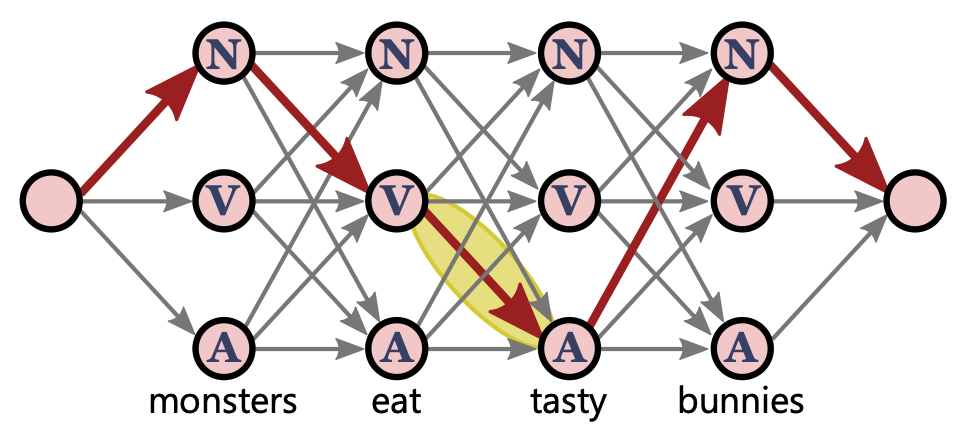
\includegraphics[height=0.4\textheight]{figures/dp}
What's the running time?
\note<.>{Let $K=\vert\sY\vert$, DP runtime $O(K^2L)$, $m$th order Markov feature has runtime $O(K^mL)$, naive runtime $O(K^L)$.}
\end{description}
\let\thefootnote\relax\footnotetext{\tiny{Figure by Daum\'e III. A course in machine learning. Figure 17.1}.}
\end{frame}

% \begin{frame}
% {The argmax problem in general}
% Efficient problem-specific algorithms:
% \begin{table}
% \begin{tabular}{llll}
% \toprule
% problem & structure & algorithm \\
% \midrule
% constituent parsing & binary trees with context-free features & CYK  \\
% dependency parsing & spanning trees with edge features & Chu-Liu-Edmonds \\
% image segmentation & 2d with adjacent-pixel features & graph cuts \\
% \bottomrule
% \end{tabular}
% \end{table}
% \pause

% General algorithm:
% \begin{itemize}
% \item Integer linear programming (ILP)
% \begin{align}
% \max_z\; a^Tz \quad \text{s.t. linear constraints on $z$}
% \end{align}
% \item $z$: indicator of substructures, \eg $\1\pc{y_i=\text{article and }y_{i+1}=\text{noun}}$
% \item constraints: $z$ must correspond to a valid structure
% \end{itemize}
% \end{frame}

% Additional resource:
% https://people.cs.umass.edu/~mccallum/papers/crf-tutorial.pdf
\begin{frame}{Conditional random field (CRF)}
\begin{itemize}
\item Recall that we can write logistic regression in a general form:
\[
p(y|x) = \frac{1}{Z(x)} \exp(w^\top \psi(x, y)).
\]
\item $Z$ is normalization constant: $Z(x) = \sum_{y \in Y} \exp(w^\top \psi(x, y))$.
\pause
\item Example: linear chain $\{y_t\}$
\item We can incorporate unary and Markov features:
$p(y|x) = \frac{1}{Z(x)} \exp(\sum_t w^\top \psi(x, y_t, y_{t-1}))$
\begin{center}
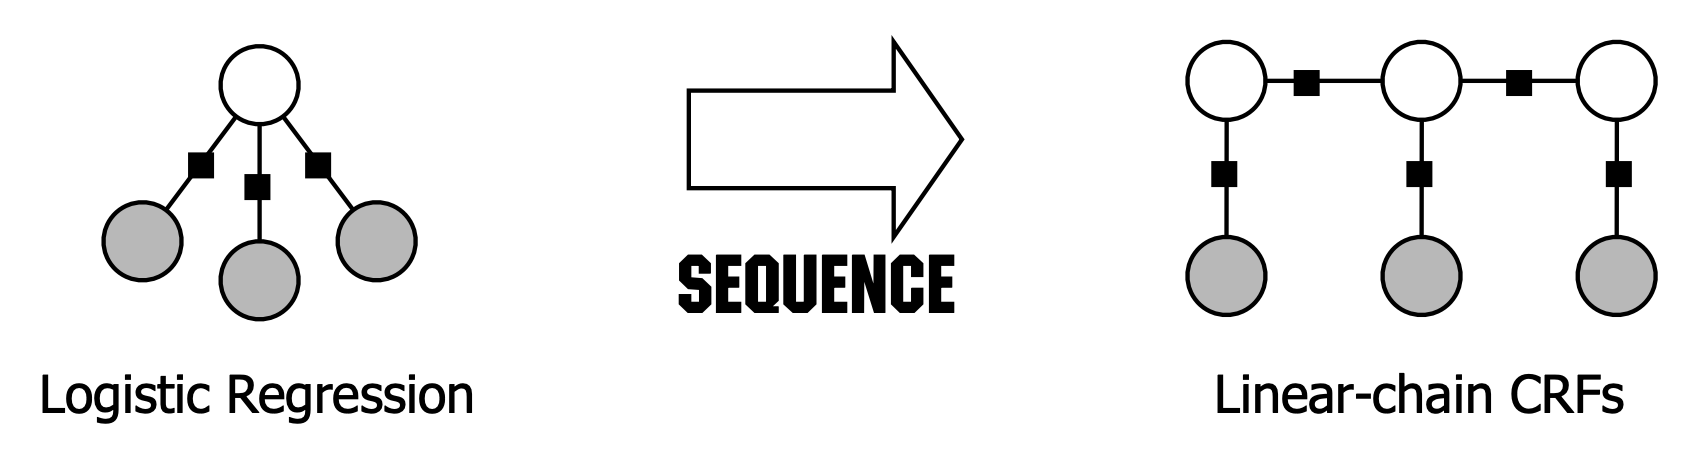
\includegraphics[width=0.6\textwidth]{figures/crf.png}
\end{center}
% \item Unary energy
% \item Pairwise energy
% \item Total energy
\end{itemize}
\end{frame}

\begin{frame}{Conditional random field (CRF)}
\begin{itemize}
  \item Compared to Structured SVM, CRF has a probabilistic interpretation.
  \item We can draw samples in the output space.
  \pause
  \item How do we learn $w$? Maximum log likelihood, and regularization term: $\lambda \lVert w \rVert^2$
  \item Loss function:
  \begin{align*}
  l(w) &= - \frac{1}{N} \sum_{i=1}^{N} \log p(y^{(i)} | x^{(i)}) + \frac{1}{2} \lambda \lVert w \rVert^2 \\
  &= - \frac{1}{N} \sum_i \sum_t \sum_k w_k \psi_k(y^{(i)}_t, y^{(i)}_{t-1}) + \frac{1}{N} \sum_{i} \log Z(x^{(i)}) + \frac{1}{2}  \sum_k \lambda w_k^2
  \end{align*}
\end{itemize}
\end{frame}

\begin{frame}{Conditional random field (CRF)}
\begin{itemize}
  \item Loss function:
  \[
  l(w)= - \frac{1}{N} \sum_i \sum_t \sum_k w_k \psi_k(x^{(i)}, y^{(i)}_t, y^{(i)}_{t-1}) + \frac{1}{N} \sum_{i} \log Z(x^{(i)}) +\frac{1}{2} \sum_k  \lambda w_k^2
  \]
\item Gradient:
\begin{align}
\frac{\partial l(w)}{\partial w_k} &= -\frac{1}{N} \sum_i \sum_t \sum_k \psi_k(x^{(i)}, y^{(i)}_t, y^{(i)}_{t-1}) \\
& + \frac{1}{N} \sum_{i} \frac{\partial}{\partial w_k} \log \sum_{y' \in Y} \exp(\sum_t \sum_{k'} w_{k'} \psi_{k'}(x^{(i)}, y'_t, y'_{t-1})) + \sum_k \lambda w_k
\end{align}
\end{itemize}
\end{frame}

\begin{frame}{Conditional random field (CRF)}
\begin{itemize}
  \item What is $\frac{1}{N} \sum_i \sum_t \sum_k \psi_k(x^{(i)}, y^{(i)}_t, y^{(i)}_{t-1})$?
  \pause

  \item It is the expectation $\psi_k (x^{(i)}, y_t, y_{t-1})$ under the empirical distribution $\tilde{p}(x, y) = \frac{1}{N} \sum_i \mathbbm{1} [x = x^{(i)}] \mathbbm{1} [y = y^{(i)}]$.
\end{itemize}
\end{frame}


\begin{frame}{Conditional random field (CRF)}
\begin{itemize}
  \item What is $\frac{1}{N} \sum_i \frac{\partial}{\partial w_k} \log \sum_{y' \in Y} \exp(\sum_t \sum_{k'} w_{k'} \psi_{k'}(x^{(i)}, y_t', y_{t-1}'))$?
  \pause
  \begin{align}
  & \frac{1}{N} \sum_i \frac{\partial}{\partial w_k} \log \sum_{y' \in Y} \exp(\sum_t \sum_{k'} w_{k'} \psi_{k'}(x^{(i)}, y_t', y_{t-1}'))\\
  &= \frac{1}{N} \sum_i \left[\sum_{y' \in Y} \exp(\sum_t \sum_{k'} w_{k'} \psi_{k'}(x^{(i)}, y_t', y_{t-1}'))\right]^{-1}\\
  &\left[\sum_{y' \in Y} \exp(\sum_t \sum_{k'} w_{k'} \psi_{k'}(x^{(i)}, y_t^{(i)}, y_{t-1}^{(i)})) \sum_t \psi_k(x^{(i)}, y_t', y_{t-1}') \right] \\
  &= \frac{1}{N} \sum_i \sum_t \sum_{y'\in Y} p(y'_t, y_{t-1}' | x) \psi_k (x^{(i)}, y'_t, y'_{t-1})
  \end{align}
  \pause
  \item It is the expectation of $\psi_k (x^{(i)}, y'_t, y'_{t-1})$ under the model distribution $p(y'_t, y_{t-1}' | x)$.
\end{itemize}
\end{frame}


\begin{frame}{Conditional random field (CRF)}
\begin{itemize}
  \item To compute the gradient, we need to infer expectation under the model distribution $p(y|x)$.
  \pause
  \item Compare the learning algorithms: in structured SVM we need to compute the argmax, whereas in CRF we need to compute the model expectation.
  \pause
  \item Both problems are NP-hard for general graphs.
\end{itemize}
\end{frame}

\begin{frame}{CRF Inference}
\begin{itemize}
  \item In the linear chain structure, we can use the forward-backward algorithm for inference, similar to Viterbi.
  \pause
  \item Initiate $\alpha_j(1) = \exp (w^\top \psi(y_1=j, x_1))$
  \pause
  \item Recursion: $\alpha_j(t) = \sum_i \alpha_i (t-1) \exp(w^\top \psi(y_t=j, y_{t-1}=i, x_t))$
  \pause
  \item Result: $Z(x) = \sum_j \alpha_j(T)$
  \pause
  \item Similar for the backward direction.
  \pause
  \item Test time, again use Viterbi algorithm to infer argmax.
  \pause
  \item The inference algorithm can be generalized to belief propagation (BP) in a tree structure (exact inference).
  \pause
  \item In general graphs, we rely on approximate inference (e.g. loopy belief propagation).
\end{itemize}
\end{frame}

\begin{frame}{Examples}
\begin{itemize}
  \item POS tag
  Relationship between constituents, e.g. NP is likely to be followed by a VP.
  \pause

  \item Semantic segmentation
  
  Relationship between pixels, e.g. a grass pixel is likely to be next to another grass pixel, and a sky pixel is likely to be above a grass pixel.
  \pause

  \item Multi-label learning

  An image may contain multiple class labels, e.g. a bus is likely to co-occur with a car.
\end{itemize}
\end{frame}

\begin{frame}
{Conclusion}
Multiclass algorithms
\begin{itemize}
\item Reduce to binary classification, \eg OvA, AvA
\begin{itemize}
\item Good enough for simple multiclass problems
\item They don't scale and have simplified assumptions
\end{itemize}
\pause
\item Generalize binary classification algorithms using multiclass loss
\begin{itemize}
\item Multi-class perceptron, multi-class logistics regression, multi-class SVM
% \item Useful for problems with extremely large output space, \eg structured prediction
% \item Related problems: ranking, multi-label classification
\end{itemize}
\pause
\item Structured prediction: Structured SVM, CRF. Data containing structure. Extremely large output space. Text and image applications.
\end{itemize}
\end{frame}

\end{document}

